\documentclass[10pt, letterpaper]{article}

% Inhaltsverzeichnis für Pakettypen (nur für Übersicht im Header, wird nicht im Dokument angezeigt)
% 1. Seitenlayout und Ränder
% 2. Sprache und Zeichensatz
% 3. Mathematik und Theorem-Umgebungen
% 4. Eigene Makros
% 5. Diagramme und Grafiken
% 6. Tabellen und Aufzählungen
% 7. Inhaltsverzeichnis
% 8. Abschnittsüberschriften
% 9. Abstrakt-Umgebung
% 10. Todos/Notizen
% 11. Rahmen/Box-Umgebungen
% 12. Python-Integration
% 13. Literaturverwaltung
% 14. Hyperlinks
% 15. Absatzeinstellungen
% 16. Umgebungen
% 17  Graphik
% 18  Extra
% 00. Titel und Autor

\usepackage{slashed}

% --- 1. Seitenlayout und Ränder ---
\usepackage[margin=3cm]{geometry}

% --- 2. Sprache und Zeichensatz ---
\usepackage[english]{babel}
\usepackage[T1]{fontenc}
\usepackage[utf8]{inputenc}

% --- 3. Mathematik und Theorem-Umgebungen ---
\usepackage{amsmath, amssymb, amsthm}
\usepackage{mathrsfs}
\DeclareMathOperator{\WF}{WF}

% --- 4. Eigene Makros ---
\usepackage{xcolor}
\newcommand{\SKP}{\langle\cdot,\cdot\rangle}
\newcommand{\R}{\mathbb{R}}
\newcommand{\N}{\mathbb{N}}
\newcommand{\Q}{\mathbb{Q}}
\newcommand{\Z}{\mathbb{Z}}
\newcommand{\C}{\mathbb{C}}
\newcommand{\entwurf}[1]{\textcolor{red}{#1}}

% --- 5. Diagramme und Grafiken ---
\usepackage{graphicx}
\graphicspath{{../../Library/Images/}}
\usepackage[export]{adjustbox}
\usepackage{tikz}
\usetikzlibrary{decorations.pathreplacing, arrows.meta, positioning}
\usepackage{tikz-cd}

% --- 6. Tabellen und Aufzählungen ---
\usepackage{enumitem}
\setlist[itemize]{left=0.5cm}

\newenvironment{romanenum}[1][]
  {%
    \ifx&#1&
    \else
      \textbf{#1}\quad
    \fi
    \begin{enumerate}[label=\roman*)]
  }
  {%
    \end{enumerate}%
  }

% --- 7. Inhaltsverzeichnis ---
\usepackage{tocloft}
\renewcommand{\cftsecfont}{\footnotesize}
\renewcommand{\cftsubsecfont}{\footnotesize}
\renewcommand{\cftsubsubsecfont}{\footnotesize}
\renewcommand{\cftsecpagefont}{\footnotesize}
\renewcommand{\cftsubsecpagefont}{\footnotesize}
\renewcommand{\cftsubsubsecpagefont}{\footnotesize}
\usepackage{etoc}

% --- 8. Abschnittsüberschriften ---
\usepackage{titlesec}
\titleformat{\section}{\normalfont\large\bfseries}{\thesection}{1em}{}
\titleformat{\subsection}{\normalfont\normalsize\bfseries}{\thesubsection}{0.5em}{}
\titleformat{\subsubsection}{\normalfont\normalsize\bfseries}{\thesubsubsection}{0.5em}{}
\setcounter{secnumdepth}{4}

% --- 9. Abstrakt-Umgebung ---
\usepackage{changepage}
\renewenvironment{abstract}
  {
    \begin{adjustwidth}{1.5cm}{1.5cm}
    \small
    \textsc{Abstract. –}%
  }
  {
    \end{adjustwidth}
  }

% --- 10. Todos/Notizen ---
\usepackage{todonotes}
% Hellblau definieren
\definecolor{hellblau}{rgb}{0.3,0.6,1}
\newenvironment{note}{\par\begingroup\color{hellblau}\itshape}{\par\endgroup}

% --- 11. Rahmen/Box-Umgebungen ---
\usepackage{mdframed}
\usepackage{tcolorbox}
\colorlet{shadecolor}{gray!25}

\newenvironment{customTheorem}
  {\vspace{10pt}%
   \begin{mdframed}[
     backgroundcolor=gray!20,
     linewidth=0pt,
     innertopmargin=10pt,
     innerbottommargin=10pt,
     skipabove=\dimexpr\topsep+\ht\strutbox\relax,
     skipbelow=\topsep,
   ]}
  {\end{mdframed}
   \vspace{10pt}%
  }

% --- 12. Python-Integration ---
% (Deaktiviert in dieser Version, aktiviere bei Bedarf)
% \usepackage{pythontex}
% \usepackage[makestderr]{pythontex}

% --- 13. Literaturverwaltung ---
\usepackage{csquotes}
\usepackage[backend=biber, style=alphabetic, citestyle=alphabetic]{biblatex}
\addbibresource{bibliography.bib}

% --- 14. Hyperlinks ---
\usepackage{hyperref}
\hypersetup{
  colorlinks   = true,
  urlcolor     = blue,
  linkcolor    = blue,
  citecolor    = blue,
  frenchlinks  = true
}

% --- 15. Absatzeinstellungen ---
\usepackage[parfill]{parskip}
\sloppy

% --- 16. Umgebungen ---
\usepackage{thmtools}

\newcommand{\CustomHeading}[3]{%
  \par\medskip\noindent%
  \textbf{#1 #2} \textnormal{(#3)}.\enskip%
}

\newenvironment{DEF}[2]{\begin{unitbox}\CustomHeading{Definition}{#1}{#2}}{\end{unitbox}}
\newenvironment{PROP}[2]{\begin{unitbox}\CustomHeading{Proposition}{#1}{#2}}{\end{unitbox}}
\newenvironment{THEO}[2]{\begin{unitbox}\CustomHeading{Theorem}{#1}{#2}}{\end{unitbox}}
\newenvironment{LEM}[2]{\begin{unitbox}\CustomHeading{Lemma}{#1}{#2}}{\end{unitbox}}
\newenvironment{KORO}[2]{\begin{unitbox}\CustomHeading{Corollar}{#1}{#2}}{\end{unitbox}}
\newenvironment{REM}[2]{\begin{unitbox}\CustomHeading{Remark}{#1}{#2}}{\end{unitbox}}
\newenvironment{EXA}[2]{\begin{unitbox}\CustomHeading{Example}{#1}{#2}}{\end{unitbox}}
\newenvironment{STUD}[2]{\begin{unitbox}\CustomHeading{Study}{#1}{#2}}{\end{unitbox}}
\newenvironment{CONC}[2]{\begin{unitbox}\CustomHeading{Concept}{#1}{#2}}{\end{unitbox}}
\newenvironment{OTH}[2]{\begin{unitbox}\CustomHeading{Other}{#1}{#2}}{\end{unitbox}}
\newenvironment{EXE}[2]{\begin{unitbox}\CustomHeading{Exercise}{#1}{#2}}{\end{unitbox}}
\newenvironment{MOT}[2]{\begin{unitbox}\CustomHeading{Motivation}{#1}{#2}}{\end{unitbox}}
\newenvironment{PROOF}[2]{\begin{unitbox}\CustomHeading{Proof}{#1}{#2}}{\end{unitbox}}

% --- Unit Umgebung für Source-Inhalte ---
\usepackage{mdframed}
\newmdenv[
  linewidth=1pt,
  topline=false,
  bottomline=false,
  rightline=false,
  leftmargin=0cm,
  rightmargin=0cm,
  skipabove=10pt,
  skipbelow=10pt,
  innertopmargin=0.5\baselineskip,
  innerbottommargin=0.5\baselineskip,
  backgroundcolor=gray!10,
  linecolor=gray
]{unitbox}

\newenvironment{unit}[1]
  {\begin{unitbox}\textbf{Unit #1}\par\smallskip}
  {\end{unitbox}}

% --- 17. ... ---

% --- 18. Extras ---
\usepackage{stmaryrd}
\usepackage{bbold}  % falls du \mathbb{1} nutzen willst

% --- 00. Titel und Autor ---
\title{Mein Titel}
\author{Tim Jaschik}
\date{\today}

\begin{document}

\maketitle
\rule{\textwidth}{0.5pt}
\begin{abstract}
Kurze Beschreibung …
\end{abstract}
\rule{\textwidth}{0.5pt}
\vspace{0.5cm}

\tableofcontents

\pagebreak


\section*{Chapter 8 Cell Complexes}
The success of algebraic topology is largely due to the fact that one can describe spaces of interest by discrete (or even finite) combinatorial data. Purely combinatorial objects are simplicial complexes. Given such a complex, one defines from its data by simple linear algebra the homology groups. It is then a remarkable fact that these groups are independent of the combinatorial description and even homotopy invariant. Simplicial complexes are a very rigid structure. A weakening of this structure is given by the cell complexes (CW-complexes in the sense of J. H. C. Whitehead). They are more flexible and better adapted to homotopy theory.

An $n$-cell in a space is a subset which is homeomorphic to the standard $n$-cell $E^{n}=\left\{x \in \mathbb{R}^{n} \mid\|x\|<1\right\}$. A cell complex is a decomposition of a space into cells. In order that one obtains something interesting, one has to add conditions about the closure of the cells, and one has to relate the topology of the space to the topology of the closed cells.

A finite cell complex is easily defined: a Hausdorff space $X$ which is the union of a finite number of cells. It $e$ is an $n$-cell of this decomposition, then it is required that there exists a continuous map $\varphi: D^{n} \rightarrow X$ which induces a homeomorphism $E^{n} \rightarrow e$ and sends $S^{n-1}$ into the union of the cells up to dimension $n-1$.

From these data one obtains already an interesting invariant of $X$, the so-called Euler characteristic. Let $n(i)$ denote the number of $i$-cells. Define the combinatorial Euler characteristic to be the alternating sum $\chi(X)=\sum_{i \geq 0}(-1)^{i} n(i)$. It is a nontrivial fact that h-equivalent finite complexes have the same Euler characteristic. The origin of the notion is the famous result of Leonhard Euler ( $\sim 1752$ ) that for a sphere $S^{2}$ each polyhedral decomposition yields the value $n(0)-n(1)+n(2)=2$.

In this chapter we present some point-set topology and elementary homotopy theory of cell complexes. Then we demonstrate the use of cell complexes in the construction of spaces with specific properties. In particular we construct so-called Eilenberg-Mac Lane spaces $K(\pi, n)$. They have a single non-vanishing homotopy group $\pi_{n}(K(\pi, n)) \cong \pi$ (here $\pi$ can be an arbitrary abelian group). Eilenberg-Mac Lane spaces can be used as building blocks for general homotopy types (Postnikov systems). They also yield a homotopical definition of cohomology (and homology) groups: The homotopy set $[X, K(\pi, n)]$ carries a natural structure of an abelian group and is known to be a version of a cohomology group denoted $H^{n}(X ; \pi)$.

\subsection*{Simplicial Complexes}
Simplicial complexes are the objects of combinatorial topology.\\
A simplicial complex $K=(E, S)$ consists of a set $E$ of vertices and a set $S$ of finite non-empty subsets of $E$. A set $s \in S$ with $q+1$ elements is called a $q$-simplex of $K$. We require the following axioms:\\
(1) $\{e\} \in S$ for each $e \in E$.\\
(2) If $t \in S$ and $s \subset t$ is non-empty, then $s \in S$.

If $s \in S$ is a $q$-simplex, then $q$ is called the dimension of $s$. If $t \subset s$, then $t$ is a face of $s$. A 1 -simplex of $K$ is also called an edge of $K$. The 0 -simplices of $K$ correspond to the elements of $E$; a 0 -simplex is called a vertex. A simplex is determined by its 0 -faces.

A simplicial complex is $n$-dimensional, if it contains at least one $n$-simplex but no ( $n+1$ )-simplices. A subcomplex $L$ of $K$ consists of a set of simplices of $K$ which contains with $s$ also the faces of $s$. A 1 -dimensional complex is a graph. A complex $K=(E, S)$ is finite if $E$ is finite and locally finite if each vertex is contained in a finite number of simplices. The $n$-skeleton $K^{n}=\left(E, S^{n}\right)$ of $K=(E, S)$ is the subcomplex with $S^{n}=\{s \in S \mid \operatorname{dim} s \leq n\}$.\\
(8.1.1) Example. Let $\mathcal{U}=\left(U_{j} \mid j \in J\right)$ be a covering of a set $X$ by nonempty sets $U_{j}$. For a finite non-empty set $E \subset J$ let $U_{E}=\bigcap_{j \in E} U_{j}$ and let $E(J)=\left\{E \subset J \mid U_{E} \neq \emptyset\right\}$. Then ( $J, E(J)$ ) is a simplicial complex, called the nerve $N(\mathcal{U})$ of the covering $\mathcal{U}$.\\
(8.1.2) Example. Let $P$ be a set with a partial ordering $\leq$. The simplicial complex ( $P, S_{P}$ ) associated to a partially ordered set has as simplices the totally ordered finite subsets of $P$.\\
(8.1.3) Example. Let $K=(E, S)$ be a simplicial complex. Define a partial order on $S$ by $s \leq t \Leftrightarrow s \subset t$. The simplicial complex $K^{\prime}$ associated to this ordered set is called the barycentric subdivision of $K$.

Let $K=(E, S)$ be a simplicial complex. We denote by $|K|$ the set of functions $\alpha: E \rightarrow I$ such that\\
(1) $\{e \in E \mid \alpha(e)>0\}$ is a simplex of $K$.\\
(2) $\sum_{e \in E} \alpha(e)=1$.

We regard $|K|$ as a subset of the product $I^{E}$. Let $|K|_{p}$ denote this set with the subspace topology of the product topology. We have a metric $d$ on $|K|$ defined by

$$
d(\alpha, \beta)=\left(\sum_{e \in E}(\alpha(e)-\beta(e))^{2}\right)^{\frac{1}{2}} .
$$

We denote $|K|$ with this metric topology by $|K|_{m}$. Each vertex $e \in E$ gives us a continuous map $e:|K|_{m} \rightarrow I, \alpha \mapsto \alpha(e)$. Therefore the identity $|K|_{m} \rightarrow|K|_{p}$ is\\
continuous. We leave it as an exercise to show that this map is actually a homeomorphism. The numbers ( $\alpha(e) \mid e \in E$ ) are the barycentric coordinates of $\alpha$.

We define a further topology on $|K|$. For $s \in S$ let $\Delta(s)$ be the standard simplex $\left\{\left(t_{e}\right) \in|K| \mid t_{e}=0\right.$ for $\left.e \notin s\right\}$. Then $|K|$ is the union of the $\Delta(s)$, and we write $|K|_{c}$ for $|K|$ with the quotient topology defined by the canonical map $\coprod_{s \in S} \Delta(s) \rightarrow|K|$. The identity $|K|_{c} \rightarrow|K|_{p}$ is continuous but not, in general, a homeomorphism. The next proposition will be proved in the more general context of simplicial diagrams.\\
(8.1.4) Proposition. $|K|_{c} \rightarrow|K|_{p}$ is a homotopy equivalence.

In the sequel we write $|K|=|K|_{c}$ and call this space the geometric realization of $K$. We define $|s| \subset|K|$ as $|s|=\{\alpha \in|K| \mid \alpha(e) \neq 0 \Rightarrow e \in s\}$ and call this set a closed simplex of $|K|$. For each simplex $s$ of $K$ the open simplex $\langle s\rangle \subset|K|$ is the subspace $\langle s\rangle=\{\alpha \in|K| \mid \alpha(e) \neq 0 \Leftrightarrow e \in s\}$. The complement $|s| \backslash\langle s\rangle=\partial|s|$ is the combinatorial boundary of $|s|$; it is the geometric realization of the subcomplex which consists of the proper faces of $s$. The set $|K|$ is the disjoint union of the $\langle s\rangle, s \in S$.

Let $|K|^{n}$ be the union of the $\Delta(s)$ with $\operatorname{dim} s \leq n$.\\
(8.1.5) Proposition. The space $|K|$ is the colimit of the $|K|^{n}$. The equality $\left|K^{n}\right|=$ $|K|^{n}$ holds. The canonical diagram\\
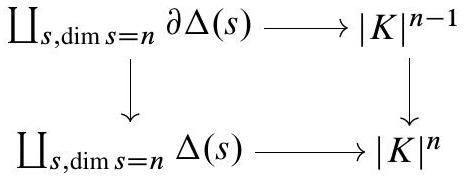
\includegraphics[scale=0.3,center]{2025_08_12_ad5732f7678306ae2ee7g-211}\\
is a pushout.\\
A homeomorphism $t:|K| \rightarrow X$ is called a triangulation of $X$. The triangulation of surfaces was proved by Radó [161], the triangulation of 3-dimensional manifolds by Moise (see [141] for references and proofs; [197, 7.5.1]). Differentiable manifolds can be triangulated, and the triangulation can be chosen in such a way that it is on each simplex a smooth embedding ([193]; [143]).

Since $|K|_{m}$ is separated and id: $|K| \rightarrow|K|_{m}$ continuous, $|K|$ is separated. For finite $K$ the identity $|K| \rightarrow|K|_{m}$ is a homeomorphism.

For each vertex $e \in E$ the set $\operatorname{St}(e)=\{\alpha \in|K| \mid \alpha(e) \neq 0\}$ is called the star of $e$. Since $\alpha \mapsto \alpha(e)$ is continuous, the set $\operatorname{St}(e)$ is open in $|K|_{d}$ and therefore also in $|K|$. If we identify $e$ with the function $\alpha(e)=1, \alpha\left(e^{\prime}\right)=0$ for $e \neq e^{\prime}$, then $\operatorname{St}(e)$ is an open neighbourhood of $e$.

Points $e_{0}, \ldots, e_{k}$ of $\mathbb{R}^{n}$ are affinely independent, if the relations $\Sigma \lambda_{i} e_{i}=0$ and $\Sigma \lambda_{i}=0$ imply that each $\lambda_{i}=0$. If $e_{0}, \ldots, e_{k}$ are affinely independent, then the simplex $\left\{\sum_{i=0}^{k} \lambda_{i} e_{i} \mid \lambda_{i} \geq 0, \Sigma \lambda_{i}=1\right\}$ spanned by $e_{0}, \ldots, e_{k}$ is the convex hull of this set and homeomorphic to the $k$-dimensional standard simplex.

Let $K=(E, S)$ be a simplicial complex and ( $x_{e} \mid e \in E$ ) a family of points in $\mathbb{R}^{n}$. Consider the continuous map

$$
f:|K| \rightarrow \mathbb{R}^{n}, \quad \alpha \mapsto \sum_{e \in E} \alpha(e) x_{e}
$$

If $f$ is an embedding, we call the image of $f$ a simplicial polyhedron in $\mathbb{R}^{n}$ of type $K$, and $f(|K|)$ is a realization of $K$ as a polyhedron in $\mathbb{R}^{n}$.

Standard tools for the application of simplicial complexes in algebraic topology are subdivision and simplicial approximation [67, p. 124].

\section*{Problems}
\begin{enumerate}
  \item id: $|K|_{m} \rightarrow|K|_{p}$ is a homeomorphism.
  \item Let $K=\left(\mathbb{N}_{0}, S\right)$ be the simplicial complex where $S$ consists of all finite subsets of $\mathbb{N}_{0}$. The canonical map $|K|_{c} \rightarrow|K|_{p}$ is not a homeomorphism.
  \item Let $L$ be a subcomplex of $K$. We can identify $|L|$ with a subset of $|K|$, and $|L|$ carries then the subspace topology of $|K|$. If ( $L_{j} \mid j \in J$ ) is a family of subcomplex of $K$, then $\bigcup L_{j}$ and $\bigcap L_{j}$ are subcomplexes and the relations $\bigcup\left|L_{j}\right|=\left|\bigcup L_{j}\right|$ and $\bigcap\left|L_{j}\right|=\left|\bigcap L_{j}\right|$ hold.
  \item Let $K$ be a simplicial complex. Then the following assertions are equivalent: (1) $K$ is locally finite. (2) $|K|$ is locally compact. (3) The identity $|K| \rightarrow|K|_{d}$ is a homeomorphism.\\
(4) $|K|$ is metrizable. (5) Each point of $|K|$ has a countable neighbourhood basis. (See [44, p. 65].)
  \item Let $K$ be a countable, locally finite simplicial complex of dimension at most $n$. Then $K$ has a realization as a polyhedron in $\mathbb{R}^{2 n+1}$. (See [44, p. 66].)
\end{enumerate}

\subsection*{Whitehead Complexes}
We use the standard subsets of Euclidean spaces $S^{n-1}, D^{n}, E^{n}=D^{n} \backslash S^{n-1}$, $(n \geq 1)$. We set $S^{-1}=\emptyset$ and let $D^{0}$ be a point, hence $E^{0}=D^{0}$. A $\boldsymbol{k}$-dimensional cell (a $k$-cell) in a space $X$ is a subset $e$ which is, in its subspace topology, homeomorphic to $E^{k}$. A point is always a 0 -cell.

A Whitehead complex is a space $X$ together with a decomposition into cells $\left(e_{\lambda} \mid \lambda \in \Lambda\right)$ such that:\\
(W1) $X$ is a Hausdorff space.\\
(W2) For each $n$-cell $e_{\lambda}$ there exists a characteristic map $\Phi_{\lambda}: D^{n}=D_{\lambda}^{n} \rightarrow X$ which induces a homeomorphism $E^{n} \rightarrow e_{\lambda}$ and sends $S^{n-1}$ into the union $X^{n-1}$ of the cells up to dimension $n-1$.\\
(W3) The closure $\bar{e}_{\lambda}$ of each cell $e_{\lambda}$ intersects only a finite number of cells.\\
(W4) $X$ carries the colimit topology with respect to the family $\left(\bar{e}_{\lambda} \mid \lambda \in \Lambda\right)$.\\
A subset $A$ of a Whitehead complex is a subcomplex if it is a union of cells and the closure of each cell in $A$ is contained in $A$. We will see that a subcomplex together with its cells is itself a Whitehead complex. From the definition of a subcomplex\\
we see that intersections and unions of subcomplexes are again subcomplexes. Therefore there exists a smallest subcomplex $X(L)$ which contains a given set $L$.

The decomposition of a Hausdorff space into its points always satisfies (W1)(W3). We see that (W4) is an important condition. Condition (W3) is also called (C), for closure finite. Condition (W4) is called (W), for weak topology. This is the origin for the name CW-complex. In the next section we consider these complexes from a different view-point and introduce the notion of a CW-complex.\\
(8.2.1) Lemma. Let $\Phi: D^{n} \rightarrow X$ be a continuous map into a Hausdorff space. Let $e=\Phi\left(E^{n}\right)$. Then $\Phi\left(D^{n}\right)=\bar{e}$. In particular $\bar{e}$ is compact.

Proof. $\Phi\left(D^{n}\right)$ is a compact subset of a Hausdorff space and therefore closed. This yields $\bar{e}=\overline{\Phi\left(E^{n}\right)} \subset \overline{\Phi\left(D^{n}\right)}=\Phi\left(D^{n}\right)=\Phi\left(\overline{E^{n}}\right) \subset \overline{\Phi\left(E^{n}\right)}=\bar{e}$.\\
(8.2.2) Example. Suppose $X$ has a cell decomposition into a finite number of cells such that properties (W1) and (W2) hold. Then $X$ is a finite union of closures $\bar{e}$ of cells and therefore compact by (8.2.1). Properties (W3) and (W4) are satisfied and $X$ is a Whitehead complex.\\
(8.2.3) Examples. The sphere $S^{n}$ has the structure of a Whitehead complex with a single 0 -cell and a single $n$-cell. The map

$$
\Phi: D^{n} \rightarrow S^{n}, \quad x \mapsto\left(2 \sqrt{1-\|x\|^{2}} \cdot x, 2\|x\|^{2}-1\right)
$$

sends $S^{n-1}$ to the 0 -cell $e_{n+1}=(0, \ldots, 0,1)$ and induces a homeomorphism of $E^{n}$ with $S^{n} \backslash\left\{e_{n+1}\right\}$, hence is a characteristic map for the $n$-cell.

From this cell decomposition we obtain a cell decomposition of $D^{n+1}$ by adding another $(n+1)$-cell $E^{n+1}$ with characteristic map the identity.

Another cell-composition of $S^{n}$ has two $j$-cells for each $j \in\{0, \ldots, n\}$ and is obtained inductively from $D_{ \pm}^{n}=\left\{\left(x_{i}\right) \in S^{n} \mid \pm x_{n+1} \geq 0\right\}$ with intersection $S^{n-1}=S^{n-1} \times 0$. A characteristic map is $D^{n} \rightarrow D_{ \pm}^{n}, x \mapsto\left(x, \pm \sqrt{1-\|x\|^{2}}\right) . \diamond$\\
(8.2.4) Proposition. Let $X$ be a Whitehead complex.\\
(1) A compact set $K$ in $X$ meets only a finite number of cells.\\
(2) A subcomplex which consists of a finite number of cells is compact and closed in $X$.\\
(3) $X(e)=X(\bar{e})$ is for each cell e a finite subcomplex.\\
(4) A compact subset of a Whitehead complex is contained in a finite subcomplex.\\
(5) $X$ carries the colimit topology with respect to the finite subcomplexes.\\
(6) A subcomplex $A$ is closed in $X$.

Proof. (1) Let $E$ be the set of cells which meet $K$. For each $e \in E$ we choose a point $x_{e} \in K \cap e$ and set $Z=\left\{x_{e} \mid e \in E\right\}$. Let $Y \subset Z$ be any subset. For each cell $f$ of $X$ the closure $\bar{f}$ is contained in the union of a finite number of cells. Thus\\
$Y \cap \bar{f}$ is a finite set, hence closed in $\bar{f}$ since $\bar{f}$ is a Hausdorff space. The condition (W4) now says that $Y$ is closed in $X$ and hence in $Z$. This tells us that $Z$ carries the discrete topology and is closed in $X$. A discrete closed set in a compact space is finite.\\
(2) Let $A=e_{1} \cup \cdots \cup e_{r}$ be a finite union of cells $e_{j}$. Then $\bar{A}=\bar{e}_{1} \cup \cdots \cup \bar{e}_{r} \subset A$, by definition of a subcomplex. By (8.2.1), $A=\bar{A}$ is compact and closed.\\
(3) Induction over $\operatorname{dim}(e)$. If $e$ is a 0 -cell, then $e$ is a point and closed, hence a subcomplex and $X(e)=X(\bar{e})=e$. Suppose $X(f)$ is finite for each cell $f$ with $\operatorname{dim}(f)<n$. Let $e$ be an $n$-cell with characteristic map $\Phi$.

The set $\Phi\left(S^{n-1}\right)$ is contained in the union of cells of dimension at most $n-1$, hence is contained in $\bar{e} \backslash e$.

Then $\bar{e} \backslash e=\Phi\left(S^{n-1}\right)$ is compact, hence contained in a finite number of cells $e_{1}, \ldots, e_{k}$, by (1), which are contained in $X^{n-1}$, by (W2). By induction hypothesis, the set $C=e \cup X\left(e_{1}\right) \cup \cdots \cup X\left(e_{k}\right)$ is a finite subcomplex which contains $e$ and hence $X(e)$. Therefore $X(e)$ is finite. Since $X(e)$ is closed, by (2), we have $\bar{e} \subset X(e)$ and $X(\bar{e}) \subset X(e)$.\\
(4) This is a consequence of (1) and (3).\\
(5) We show: $A \subset X$ is closed if and only if for each finite subcomplex $Y$ the intersection $A \cap Y$ is closed in $Y$.

Suppose the condition is satisfied, and let $f$ be an arbitrary cell. Then $\underline{A} \cap X(f)$ is closed in $X(f)$, hence, by (2) and (3), closed in $X$; therefore $A \cap \bar{f}=A \cap$ $X(f) \cap \bar{f}$ is closed in $X$ and in $\bar{f}$, hence closed in $X$ by condition (W4).\\
(6) If $Y$ is a finite subcomplex, then $A \cap Y$ is a finite subcomplex, hence closed. By (5), $A$ is closed.\\
(8.2.5) Proposition. A subcomplex $Y$ of a Whitehead complex $X$ is a Whitehead complex.

Proof. Let $e$ be a cell in $Y$ and $\Phi: D^{n} \rightarrow X$ a characteristic map. Then $\Phi\left(D^{n}\right)=$ $\bar{e} \subset Y$, since $Y$ is closed. Hence $\Phi$ can be taken as a characteristic map for $Y$.

It remains to verify condition (W4). Let $L \subset Y$ and suppose $L \cap \bar{e}$ is closed in $\bar{e}$ for each cell $e$ in $Y$. We have to show that $L$ is closed in $Y$. We show that $L$ is closed in $X$. Let $f$ be a cell of $X$. By (W3), $\bar{f}$ is contained in a finite union $e_{1} \cup \cdots \cup e_{k}$ of cells. Let $e_{1}, \ldots, e_{j}$ be those which are contained in $Y$. Then

$$
\bar{f} \cap Y \subset e_{1} \cup \cdots \cup e_{j} \subset \bar{e}_{1} \cup \cdots \cup \bar{e}_{j} \subset Y
$$

since $Y$ is a subcomplex. Hence\\
$\bar{f} \cap Y=\left(\bar{f} \cap \bar{e}_{1}\right) \cup \cdots \cup\left(\bar{f} \cap \bar{e}_{j}\right), \quad \bar{f} \cap L=\bar{f} \cap L \cap Y=\bigcup_{k=1}^{j}\left(\bar{f} \cap \bar{e}_{k} \cap L\right)$.\\
By assumption, $\bar{e}_{k} \cap L$ is closed in $\bar{e}_{k}$; hence $\bar{f} \cap \bar{e}_{k} \cap L$ is closed in $\bar{f}$; therefore $\bar{f} \cap L$ is a finite union of sets which are closed in $X$.\\
(8.2.6) Proposition. Let $X$ be a Whitehead complex. Then:\\
(1) $X$ carries the colimit topology with respect to the family $\left(X^{n} \mid n \in \mathbb{N}_{0}\right)$.\\
(2) Let $\left(e_{\lambda} \mid \lambda \in \Lambda(n)\right)$ be the family of $n$-cells of $X$ with characteristic maps $\Phi_{\lambda}: D_{\lambda}^{n} \rightarrow X^{n}$ and restrictions $\varphi_{\lambda}: S_{\lambda}^{n-1} \rightarrow X^{n-1}$. Then\\
\includegraphics[scale=0.3,center]{2025_08_12_ad5732f7678306ae2ee7g-215}\\
is a pushout in TOP. ( $X^{-1}=\emptyset$.)\\
Proof. (1) Suppose $A \cap X^{n}$ is closed in $X^{n}$ for each $n$. Then for each $n$-cell $e$ of $X$ the set $A \cap \bar{e}=A \cap \bar{e} \cap X^{n}$ is closed in $\bar{e}$. By (W4), $A$ is closed in $X$.\\
(2) The diagram is a pushout of sets. Give $X^{n}$ the pushout topology and denote this space by $Z$. By construction, the identity $\kappa: Z \rightarrow X^{n}$ is continuous. We show that $\kappa$ is also closed. Let $V \subset Z$ be closed. By definition of the pushout topology this means:\\
(i) $V \cap X^{n-1}$ is closed in $X^{n-1}$.\\
(ii) $\Phi^{-1}(V) \cap D_{\lambda}^{n}$ is closed in $D_{\lambda}^{n}$, hence also compact.

We conclude that $\Phi\left(\Phi^{-1}(V) \cap D_{\lambda}^{n}\right)=V \cap \Phi\left(D_{\lambda}^{n}\right)=V \cap \bar{e}_{\lambda}$ is closed in $\bar{e}_{\lambda}$, being a continuous image of a compact space in a Hausdorff space. From (i) and (ii) we therefore conclude that for each cell $e$ of $X^{n}$ the set $V \cap \bar{e}$ is closed in $\bar{e}$. Since $X^{n}$ is a Whitehead complex, $V$ is closed in $X^{n}$.\\
(8.2.7) Proposition. Let $X$ be a Whitehead complex, pointed by a 0 -cell. The inclusions of the finite pointed subcomplexes $F \subset X$ induce a canonical map $\operatorname{colim}_{F} \pi_{k}(F, *) \rightarrow \pi_{k}(X, *)$. This map is an isomorphism.

Recall from Section 7.9 the notion of a k -space and the k -space $k(X)$ obtained from a space $X$.\\
(8.2.8) Proposition. Let $X$ have a cell decomposition such that (W1)-(W3) hold and such that each compact set is contained in a finite number of cells. Then $k(X)$ is a Whitehead complex with respect to the given cell decomposition and the same characteristic maps. Moreover, $X$ is a Whitehead complex if and only if $k(X)=X$.

Proof. Let $\Phi: D^{n} \rightarrow X$ be a characteristic map for the cell $e$. Since $\bar{e}$ is compact it has the same topology in $k(X)$. Hence $\Phi: D^{n} \rightarrow k(X)$ is continuous. Since $\Phi$ is a quotient map and $\Phi^{-1}(e)=E^{n}$, we see that $e$ has the same topology in $k(X)$ and $X$. Thus $e$ is a cell in $k(X)$ with characteristic map $\Phi$.

Let $A \cap \bar{e}$ be closed in $\bar{e}$ for each cell $e$. Let $K \subset k(X)$ be compact. By hypothesis, $K$ is contained in a finite number of cells, say $K \subset e_{1} \cup \cdots \cup e_{k}$. Then $A \cap K=\left(\left(A \cap \bar{e}_{1}\right) \cup \cdots \cup\left(A \cap \bar{e}_{k}\right)\right) \cap K$ is closed in $K$. Hence $A$ is $k$-closed.

Let $X$ and $Y$ be Whitehead complexes and $e \subset X, f \subset Y$ cells. Then $e \times f \subset X \times Y$ is a cell. From characteristic maps $\Phi: D^{m} \rightarrow X, \Psi: D^{n} \rightarrow Y$ for $e, f$ we obtain $\Phi \times \Psi: D^{m} \times D^{n} \rightarrow X \times Y$, and this can be considered as a characteristic map for $e \times f$. For this purpose use a homeomorphism

$$
\left(D^{m+n}, S^{m+n-1}\right) \rightarrow\left(D^{m} \times D^{n}, D^{m} \times S^{n-1} \cup S^{m-1} \times D^{n}\right) .
$$

With this cell structure, $X \times Y$ satisfies conditions (W1)-(W3) in the definition of a Whitehead complex. In general, property (W4) may not hold. In this case one re-topologizes $X \times Y$ such that the compact subsets do not change. The space $X \times_{k} Y=k(X \times Y)$ is then a Whitehead complex (see (8.2.8)).

\section*{Problems}
\begin{enumerate}
  \item $\mathbb{R}$ carries the structure of a Whitehead complex with 0 -cells $\{n\}, n \in \mathbb{Z}$ and 1 -cells $] n, n+1\left[, n \in \mathbb{Z}\right.$. There is an analogous Whitehead complex structure $W(\delta)$ on $\mathbb{R}^{n}$ with 0 -cells the set of points $\delta\left(k_{1}, \ldots, k_{n}\right), k_{j} \in \mathbb{Z}, \delta>0$ fixed and the associated $\delta$-cubes. Thus, given a compact set $K \subset \mathbb{R}^{n}$ and a neighbourhood $U$ of $K$, there exists another neighbourhood $L$ of $K$ contained in $U$ such that $L$ is a subcomplex of the complex $W(\delta)$. In this sense, compact subsets can be approximated by finite complexes.
  \item The geometric realization of a simplicial complex is a Whitehead complex.
\end{enumerate}

\subsection*{CW-Complexes}
We now use (8.2.6) as a starting point for another definition of a cell complex. Let ( $X, A$ ) be a pair of spaces. We say, $X$ is obtained from $A$ by attaching an $\boldsymbol{n}$-cell, if there exists a pushout\\
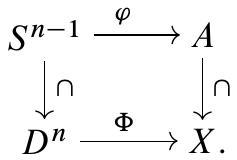
\includegraphics[scale=0.3,center]{2025_08_12_ad5732f7678306ae2ee7g-216}

Then $A$ is closed in $X$ and $X \backslash A$ is homeomorphic to $E^{n}$ via $\Phi$. We call $X \backslash A$ an $\boldsymbol{n}$-cell in $X, \varphi$ its attaching map and $\Phi$ its characteristic map.\\
(8.3.1) Proposition. Let a commutative diagram with closed embeddings $j, J$ be given:\\
\includegraphics[scale=0.3,center]{2025_08_12_ad5732f7678306ae2ee7g-216(1)}

Suppose $F$ induces a bijection $X \backslash A \rightarrow Z \backslash Y$. Then the diagram is a pushout, provided that (1) $F(X) \subset Z$ is closed; (2) $F: X \rightarrow F(X)$ is a quotient map. Condition (2) holds if $X$ is compact and $Z$ Hausdorff.

Proof. Let $g: X \rightarrow U$ and $h: Y \rightarrow U$ be given such that $g j=h f$. The diagram is a set-theoretical pushout. Therefore there exists a unique set map $\varphi: Z \rightarrow U$ with $\varphi F=g, \varphi J=h$. Since $J$ is a closed embedding, $\varphi \mid J(Y)$ is continuous. Since $F$ is a quotient map, $\varphi \mid F(X)$ is continuous. Thus $\varphi$ is continuous, since $F(X)$ and $J(Y)$ are closed sets which cover $Z$.\\
(8.3.2) Note. Let $X$ be a Hausdorff space and $A$ a closed subset. Suppose there exists a continuous map $\Phi: D^{n} \rightarrow X$ which induces a homeomorphism $\Phi: E^{n} \rightarrow$ $X \backslash A$. Then $X$ is obtained from $A$ by attaching an $n$-cell.

Proof. We show $\Phi\left(S^{n-1}\right) \subset A$. Suppose there exists $s \in S^{n-1}$ with $\Phi(s) \in X \backslash A$. Then there exists a unique $t \in E^{n}$ with $\Phi(s)=\Phi(t)$. Let $V \subset E^{n}, W \subset D^{n}$ be disjoint open neighbourhoods of $t, s$. Then $\Phi(V) \subset X \backslash A$ is open in $X$, since $\Phi: E^{n} \rightarrow X \backslash A$ is a homeomorphism and $A$ is closed in $X$. Since $\Phi$ is continuous, there exists an open neighbourhood $W_{1} \subset W$ of $s$ with $\Phi\left(W_{1}\right) \subset \Phi(V)$. This contradicts the injectivity of $\Phi \mid E^{n}$.

Thus $\Phi$ provides us with a map $\varphi: S^{n-1} \rightarrow A$. We now use (8.3.1).\\
(8.3.3) Example. The projective space $\mathbb{R} P^{n}$ is obtained from $\mathbb{R} P^{n-1}$ by attaching an $n$-cell. The projective space $\mathbb{C} P^{n}$ is obtained from $\mathbb{C} P^{n-1}$ by attaching a $2 n$ cell.

We recall that $\mathbb{C} P^{n-1}$ is obtained from $S^{2 n-1}$ by the equivalence relation $\left(z_{1}, \ldots, z_{n}\right) \sim\left(\lambda z_{1}, \ldots, \lambda z_{n}\right), \lambda \in S^{1}$, or from $\mathbb{C}^{n} \backslash 0$ by $z \sim \lambda z, \lambda \in \mathbb{C}^{*}$. The class of $z$ is denoted $\left[z_{1}, \ldots, z_{n}\right]$. A characteristic map $\Phi: D^{2 n} \rightarrow \mathbb{C} P^{n}$ is $x \mapsto\left[x, \sqrt{1-\|x\|^{2}}\right]$.

The space $\mathbb{R} P^{n-1}$ is obtained from $S^{n-1}$ by the relation $z \sim-z$, or from $\mathbb{R}^{n} \backslash 0$ by $z \sim \lambda z, \lambda \in \mathbb{R}^{*}$. A characteristic map $\Phi: D^{n} \rightarrow \mathbb{R} P^{n}$ is given by the same formula as in the complex case.

We can also attach several $n$-cells simultaneously. We say $X$ is obtained from $A$ by attaching $\boldsymbol{n}$-cells if there exists a pushout\\
\includegraphics[scale=0.3,center]{2025_08_12_ad5732f7678306ae2ee7g-217}

The index $j$ just enumerates different copies of the same space. Again, $A$ is then closed in $X$ and $\Phi$ induces a homeomorphism of $\coprod_{j} E_{j}^{n}$ with $X \backslash A$. Therefore $X \backslash A$ is a union of components and each component is an $n$-cell. (By invariance of dimension, the integer $n$ is determined by $X \backslash A$.) We allow $J=\emptyset$; in that case $A=X$. We write $\Phi_{j}=\Phi \mid D_{j}^{n}$ and $\varphi_{j}=\varphi \mid S^{n-1}$ and call $\Phi_{j}$ the characteristic map of the $n$-cell $\Phi\left(E_{j}^{n}\right)$ and $\varphi_{j}$ its attaching map.

Let us give another interpretation: $X=X(\varphi)$ is the double mapping cylinder of $J \stackrel{\mathrm{pr}}{\longleftrightarrow} S^{n} \times J \xrightarrow{\varphi} A$ where $J$ is a discrete set. From this setting we see: If $\varphi$ is replaced by a homotopic map $\psi$, then $X(\varphi)$ and $X(\psi)$ are h-equivalent under $A$.

Let $f: A \rightarrow Y$ be a given map. Assume that $X$ is obtained from $A$ by attaching $n$-cells via attaching maps $\left\langle\varphi_{j}\right\rangle: \coprod_{j} S_{j}^{n-1} \rightarrow A$. From the pushout definition of the attaching process we obtain:\\
(8.3.4) Note. There exists an extension $F: X \rightarrow Y$ of $f$ if and only if the maps $f \varphi_{j}$ are null homotopic. We view a null homotopy of $f \varphi_{j}$ as an extension to $D_{j}^{n}$. Then the extensions $F$ correspond to the set of null homotopies of the $f \varphi_{j}$.

In view of this note we call the homotopy classes [ $f \varphi_{j}$ ] the obstructions to extending $f$.

Let $A$ be a subspace of $X$. ACW-decomposition of ( $X, A$ ) consists of a sequence of subspaces $A=X^{-1} \subset X^{0} \subset X^{1} \subset \cdots \subset X$ such that:\\
(1) $X=\cup_{n \geq 0} X^{n}$.\\
(2) For each $n \geq 0$, the space $X^{n}$ is obtained from $X^{n-1}$ by attaching $n$-cells.\\
(3) $X$ carries the colimit topology with respect to the family $\left(X^{n}\right)$.\\
$X_{k}$ is a subspace of the colimit $X$ of a sequence $X_{j} \subset X_{j+1} \subset \cdots$. If the inclusions are closed, then $X_{k}$ is closed in $X$. This is an immediate consequence of the definition of the colimit topology.

A pair ( $X, A$ ) together with a CW -decomposition ( $X^{n} \mid n \geq-1$ ) is called a relative $\boldsymbol{C} \boldsymbol{W}$-complex. In the case $A=\emptyset$ we call $X$ a $\boldsymbol{C} \boldsymbol{W}$-complex. The space $X^{n}$ is the $n$-skeleton of ( $X, A$ ) and ( $X^{n} \mid n \geq-1$ ) is the skeleton filtration. The cells of $X^{n} \backslash X^{n-1}$ are the $n$-cells of ( $X, A$ ). We say, ( $X, A$ ) is finite (countable etc.) if $X \backslash A$ consists of a finite (countable etc.) number of cells. If $X=X^{n}, X \neq X^{n-1}$ we denote by $n=\operatorname{dim}(X, A)$ the cellular dimension of ( $X, A$ ). If $A=\emptyset$, then $A$ is suppressed in the notation. We call $X$ a $\boldsymbol{C W}$-space if there exists some cellular decomposition $X^{0} \subset X^{1} \subset \cdots$ of $X$.

Let $X$ be a Whitehead complex. From (8.2.6) we obtain a CW-decomposition of $X$. The converse also holds: From a CW-decomposition we obtain a decomposition into cells and characteristic maps; it remains to verify that $X$ is a Hausdorff space and carries the colimit topology with respect to the closures of cells (see (8.3.8)).

In the context of CW-complexes ( $X, A$ ), the symbol $X^{n}$ usually denotes the $n$-skeleton and not the $n$-fold Cartesian product.\\
(8.3.5) Note. If ( $X, A$ ) is a relative $C W$-complex, then also ( $X, X^{n}$ ) and ( $X^{n}, A$ ) are relative $C W$-complexes, with the obvious skeleton-filtration inherited from ( $X^{n} \mid n \geq-1$ ).\\
(8.3.6) Example. From (8.3.3) we obtain cellular decompositions of $\mathbb{C} P^{n}$ and $\mathbb{R} P^{n}$. The union of the sequence $\mathbb{R} P^{n} \subset \mathbb{R}^{n+1} \subset \cdots$ defines the infinite projective\\
space $\mathbb{R} P^{\infty}$ as a CW-complex. It has a single $n$-cell for each $n \geq 0$. Similarly, we obtain $\mathbb{C} P^{\infty}$ with a single cell in each even dimension.\\
(8.3.7) Example. The sphere $S^{n}$ has a CW-decomposition with a single 0 -cell and a single $n$-cell, and another CW-composition with two $j$-cells for each $j \in$ $\{0, \ldots, n\}$, see (8.2.3). The quotient map $S^{n} \rightarrow \mathbb{R} P^{n}$ sends each cell of the latter homeomorphically onto a cell of $\mathbb{R} P^{n}$ in the decomposition (8.3.6). We can also form the colimit $S^{\infty}$ of $S^{n} \subset S^{n+1} \subset \cdots$, a CW-complex with two cells in each dimension.

The general topology of adjunction spaces and colimit topologies gives us the next results.\\
(8.3.8) Proposition. Let $(X, A)$ be a relative $C W$-complex. If $A$ is a $T_{1}$-space, then $X$ is a $T_{1}$-space and a compact subset of $X$ meets only a finite number of cells. If $A$ is a Hausdorff space, then $X$ is a Hausdorff space. If $A$ is normal, then $X$ is normal. If $A$ is a Hausdorff space, then $X$ carries the colimit topology with respect to the family which consists of $A$ and the closures of cells.

Proof. We only verify the last statement. Let $C$ be a subset of $X$ and suppose $A \cap C$ in closed in $A$ and $A \cap \bar{e}$ closed in $\bar{e}$ for each cell $e$. We show inductively, that $C \cap X^{n}$ is closed in $X^{n}$. This holds for $n=-1$ by assumption. The space $X^{n}$ is a quotient of $Z^{n}=X^{n-1}+\coprod D_{j}^{n}$. Each characteristic map $\Phi_{j}: D_{j}^{n} \rightarrow \bar{e}_{j}$ is a quotient map, since $X$ is Hausdorff. From the assumptions we see that $X^{n} \cap C$ has a closed pre-image in $Z^{n}$.

The considerations so far show that a CW-complex is a Whitehead complex.\\
(8.3.9) Proposition. Let ( $X, A$ ) be a relative $C W$-complex. Then $A \subset X$ is a cofibration.

Proof. We know that $\amalg S_{j}^{n-1} \rightarrow \amalg D_{j}^{n}$ is a cofibration. Hence $X^{n-1} \subset X^{n}$ is an induced cofibration. Therefore the compositions $X^{n} \subset X^{n+k}$ are cofibrations. Given $f: X \rightarrow Z$ and a homotopy $h^{-1}: X^{-1} \times I \rightarrow Z$ of $f \mid X^{-1}$, we can extend this inductively to homotopies $h^{n}: X^{n} \times I \rightarrow Z$ such that $h^{n+1} \mid X^{n} \times I=h^{n}$. Since $X \times I$ is the colimit of the $X^{n} \times I$, the $h^{n}$ combine to a homotopy $h: X \times I \rightarrow Z$.

\section*{Problems}
\begin{enumerate}
  \item The attaching map for the $n$-cells yields a homeomorphism $\bigvee_{j}\left(D^{n} / S^{n-1}\right)_{j} \cong X / A$.
  \item Let ( $X, A$ ) and ( $Y, B$ ) be relative CW-complexes. Consider $X \times Y$ with the closed subspaces
\end{enumerate}

$$
(X \times Y)^{n}=\bigcup_{i=-1}^{n+1} X^{i} \times Y^{n-i}, \quad n \geq-1 .
$$

In favorable cases, the filtration $\left((X \times Y)^{n} \mid n \geq-1\right)$ is a CW-decomposition of the pair $(X \times Y, A \times B)$.

Let $Y$ be locally compact. Then $(X \times Y)^{n}$ is obtained from $(X \times Y)^{n-1}$ by attaching $n$-cells.\\
3. Let ( $X, A$ ) be a relative CW -complex and let $C \subset A$. Then ( $X / C, A / C$ ) is a relative CW-complex with CW-decomposition $\left(X^{n} / C\right)$. Moreover, $X / A$ is a CW-complex.\\
4. Let $A \subset X$ be a subcomplex. Then $X / A$ is a CW-complex.\\
5. Let $A$ and $B$ be subcomplexes of $X$. Then $A /(A \cap B)$ is a subcomplex of $X / B$.\\
6. Let $A$ be a subcomplex of $B$ and $Y$ another CW-complex. Then $A \wedge_{k} Y$ is a subcomplex of $B \wedge_{k} Y$.\\
7. Let $A$ be a CW-complex. Suppose $X$ is obtained from $A$ by attaching $n$-cells via attaching maps $\varphi$ : $\amalg S_{j}^{n-1} \rightarrow A^{n-1}$. Then $X$ is a CW-complex with CW-decomposition $X^{j}=A^{j}$ for $j<n$ and $X^{j}=A^{j} \cup(X \backslash A)$ for $j \geq n$, and $A$ is a subcomplex of $X$.\\
8. Let $\varphi_{0}, \varphi_{1}: \amalg, S_{j}^{n-1} \rightarrow A$ be homotopic attaching maps. The spaces $X(0), X(1)$ which are obtained by attaching $n$-cells with $\varphi_{0}, \varphi_{1}$ are h-equivalent under $A$. (Homotopy theorem for cofibrations.)\\
9. Let $X$ be a pointed CW-complex with base point $*$ a 0 -cell. Then the cone $C X$ and the suspension $\Sigma X$ are CW-complexes. (In statements of this type the reader is asked to find a canonical cell decomposition induced from the initial data.)\\
10. Let $\left(X_{j} \mid j \in J\right)$ be a family of pointed CW-complexes with base point a 0 -cell. Then $\bigvee_{j \in J} X_{j}$ has the structure of a CW-complex such that the summands are subcomplexes.\\
11. Let $p: E \rightarrow B$ be a Serre fibration and ( $X, A$ ) a CW-pair. Then each homotopy $h: X \times I \rightarrow B$ has a lifting along $p$ with given initial condition on $X \times 0 \cup A \times I$.\\
12. Suppose $X$ is obtained from $A$ by attaching $n$-cells. Let $p: E \rightarrow X$ be a covering and $E^{\prime}=p^{-1}(A)$. Then $E$ is obtained from $E^{\prime}$ by attaching $n$-cells.\\
13. Let $X$ be a CW-complex with $n$-skeleton $X^{n}$ and $p: E \rightarrow X$ a covering. Then $E$ is a CW-complex with $n$-skeleton $E^{n}=p^{-1}\left(B^{n}\right)$ such that $p$ maps the cells of $E$ homeomorphically to cells of $X$. An automorphism of $p$ maps cells of $E$ homeomorphically to cells.\\
14. Each neighbourhood $U$ of a point $x$ of a CW-complex contains a neighbourhood $V$ which is pointed contractible to $x$. A connected CW-complex has a universal covering. The universal covering has a cell decomposition such that its automorphism group permutes the cells freely.\\
15. Let $X$ and $Y$ be countable CW-complexes. Then $X \times Y$ is a CW-complex in the product topology.

\subsection*{Weak Homotopy Equivalences}
We now study the notion of an $n$-connected map and of a weak homotopy equivalence in the context of CW-complexes.\\
(8.4.1) Proposition. Let $(Y, B)$ be $n$-connected. Then a map $f:(X, A) \rightarrow(Y, B)$ from a relative $C W$-complex $(X, A)$ of dimension $\operatorname{dim}(X, A) \leq n$ is homotopic\\
relative to $A$ to a map into $B$. In the case that $\operatorname{dim}(X, A)<n$ the homotopy class of $X \rightarrow B$ is unique relative to $A$.

Proof. Induction over the skeleton filtration. Suppose $X$ is obtained from $A$ by attaching $q$-cells via $\varphi: \amalg_{k} S_{k}^{q-1} \rightarrow A, q \leq n$. Consider a commutative diagram\\
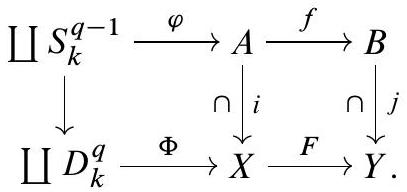
\includegraphics[scale=0.3,center]{2025_08_12_ad5732f7678306ae2ee7g-221}

Since ( $Y, B$ ) is $n$-connected, $F \Phi$ is homotopic relative to $\bigsqcup S_{k}^{q-1}$ to a map into $B$. Since the left square is a pushout, we obtain a homotopy of $F$ from a pair of homotopies of $F \Phi$ and $F i$ which coincide on $\amalg S_{k}^{q-1}$. Since we have homotopies of $F \Phi$ relative to $\amalg S_{k}^{q-1}$, we can use on $A$ the constant homotopy. Altogether we obtain a homotopy of $F$ relative to $A$ to a map into $B$.

For an arbitrary ( $X, A$ ) with $\operatorname{dim}(X, A) \leq n$ we apply this argument inductively. Suppose we have a homotopy of $f$ relative to $A$ to a map $g$ which sends $X^{k}$ into $B$. By the argument just given we obtain a homotopy of $g \mid X^{k+1}$ relative to $X^{k}$ which sends $X^{k+1}$ into $B$. Since $X^{k+1} \subset X$ is a cofibration, we extend this homotopy to $X$. In the case that $n=\infty$, we have to concatenate an infinite number of homotopies. We use the first homotopy on $[0,1 / 2]$ the second on $[1 / 2,3 / 4]$ and so on. (Compare the proof of (8.5.4).) Suppose $\operatorname{dim}(X, A)<n$. Let $F_{0}, F_{1}: X \rightarrow$ $B$ be homotopic relative to $A$ to $f$. We obtain from such homotopies a map $(X \times I, X \times \partial I \cup A \times I) \rightarrow(Y, B)$ which is the constant homotopy on $A$. We apply the previous argument to the pair $(X \times I, X \times \partial I \cup A \times I)$ of dimension $\leq n$ and see that the homotopy class of the deformation $X \rightarrow B$ of $f$ is unique relative to $A$.\\
(8.4.2) Theorem. Let $h: B \rightarrow Y$ be $n$-connected, $n \geq 0$. Then $h_{*}:[X, B] \rightarrow$ $[X, Y]$ is bijective (surjective) if $X$ is a $C W$-complex with $\operatorname{dim} X<n(\operatorname{dim} X \leq n)$. If $h: B \rightarrow Y$ is pointed, then $h_{*}:[X, B]^{0} \rightarrow[X, Y]^{0}$ is injective (surjective) in the same range.

Proof. By use of mapping cylinders we can assume that $h$ is an inclusion. The surjectivity follows if we apply (8.4.1) to the pair ( $X, \emptyset$ ). The injectivity follows, if we apply it to the pair ( $X \times I, X \times \partial I$ ). In the pointed case we deform ( $X, *$ ) $\rightarrow$ $(Y, B)$ rel $\{*\}$ to obtain surjectivity, and for the proof of injectivity we apply (8.4.1) to the pair $(X \times I, X \times \partial I \cup * \times I)$.\\
(8.4.3) Theorem. Let $f: Y \rightarrow Z$ be a map between $C W$-complexes.\\
(1) $f$ is a homotopy equivalence, if and only if for each $b \in Y$ and each $q \geq 0$ the induced map $f_{*}: \pi_{q}(Y, b) \rightarrow \pi_{q}(Z, f(b))$ is bijective.\\
(2) Suppose $\operatorname{dim} Y \leq k, \operatorname{dim} Z \leq k$. Then $f$ is a homotopy equivalence if $f_{*}$ is bijective for $q \leq k$.

Proof. (1) If $f_{*}$ is always bijective, then $f_{*}$ is a weak equivalence, hence the induced map $f_{*}:[X, Y] \rightarrow[X, Z]$ is bijective for all CW-complexes $X$ (see (8.4.2)). By category theory, $f$ represents an isomorphism in h-TOP: Take $X=Z$; then there exists $g: Z \rightarrow Y$ such that $f g \simeq \operatorname{id}(Z)$. Then $g_{*}$ is always bijective. Hence $g$ also has a right homotopy inverse.\\
(2) $f_{*}:[Z, Y] \rightarrow[Z, Z]$ is surjective, since $f$ is $k$-connected (see (8.4.2)). Hence there exists $g: Z \rightarrow Y$ such that $f g \simeq \operatorname{id}(Z)$. Then $g_{*}: \pi_{q}(Z) \rightarrow \pi_{q}(Y)$ is bijective for $q \leq k$, since $f_{*} g_{*}=\mathrm{id}$ and $f_{*}$ is bijective. Hence there exists $h: Y \rightarrow Z$ with $g h \simeq \operatorname{id}(Y)$. Thus $g$ has a left and a right h-inverse and is therefore an h-equivalence. From $f g \simeq$ id we then conclude that $f$ is an h-equivalence.

The importance of the last theorem lies in the fact that "homotopy equivalence" can be tested algebraically. Note that the theorem does not say: If $\pi_{q}(Y) \cong \pi_{q}(Z)$ for each $q$, then $Y$ and $Z$ are homotopy equivalent; it is important to have a map which induces an isomorphism of homotopy groups. Mapping a space to a point gives:\\
(8.4.4) Corollary. A CW-complex $X$ is contractible if and only if $\pi_{q}(X)=0$ for $q \geq 0$.\\
(8.4.5) Example. From $\pi_{j}\left(S^{n}\right)=0$ for $j<n$ and $\pi_{j}\left(S^{\infty}\right)=\operatorname{colim}_{n} \pi_{j}\left(S^{n}\right)$ we conclude that the homotopy groups of $S^{\infty}$ are trivial. Hence $S^{\infty}$ is contractible.

$$
\diamond
$$

(8.4.6) Example. A simply connected 1 -dimensional complex is contractible. A contractible 1-dimensional CW-complex is called a tree.\\
(8.4.7) Theorem. A connected $C W$-complex $X$ contains a maximal (with respect to inclusion) tree as subcomplex. A tree in $X$ is maximal if and only if it contains each 0-cell.

Proof. Let $\mathscr{B}$ denote the set of all trees in $X$, partially ordered by inclusion. Let $\mathcal{T} \subset B$ be a totally ordered subset. Then $C=\bigcup_{T \in \mathcal{T}} T$ is contractible: $\pi_{1}(C)=0$, since a compact subset of $C$ is contained in a finite subcomplex and therefore in some $T \in \mathcal{T}$. Thus, by Zorn's lemma, there exist maximal trees.

Let $B$ be a maximal tree. Consider the 1 -cells which have at least one end point in $B$. If the second end point is not contained in $B$, then $B$ is obviously not maximal. Therefore the union $V$ of these 1-cells together with $B$ form a subcomplex of $X^{1}$, and the remaining 1-cells together with their end points form a subcomplex $X^{1} \backslash V$. Since $X$ is connected so is $X^{1}$, hence $V=X^{1}$, and $B^{0}=V^{0}=X^{0}$.

Let $B$ be a tree which contains $X^{0}$. Let $B^{\prime} \supset B$ be a strictly larger tree. Since $B$ is contractible, $B^{\prime}$ and $B^{\prime} / B$ are h-equivalent. Hence $B^{\prime} / B$ is contractible. Since $X^{0} \subset B$, the space $B^{\prime} / B$ has the form $\bigvee S^{1}$ and is not simply connected. Contradiction.

We now generalize the suspension theorem (6.10.4). Let $X$ and $Y$ be pointed spaces. We have the suspension map $\Sigma_{*}:[X, Y]^{0} \rightarrow[\Sigma X, \Sigma Y]^{0}$. We use the adjunction $[\Sigma X, \Sigma Y]^{0} \cong[X, \Omega \Sigma Y]^{0}$. The resulting map $[X, Y]^{0} \rightarrow[X, \Omega \Sigma Y]^{0}$ is then induced by the pointed map $\sigma: Y \rightarrow \Omega \Sigma Y$ which assigns to $y \in Y$ the loop $t \mapsto[y, t]$ in $\Sigma Y$.\\
(8.4.8) Theorem. Suppose $\pi_{i}(Y)=0$ for $0 \leq i \leq n$. Then the suspension $\Sigma_{*}:[X, Y]^{0} \rightarrow[\Sigma X, \Sigma Y]^{0}$ is bijective (surjective) if $X$ is a $C W$-complex of dimension $\operatorname{dim} X \leq 2 n(\operatorname{dim} X \leq 2 n+1)$.

Proof. By the suspension theorem (6.10.4), the map $\sigma$ is $(2 n+1)$-connected. Now use the pointed version of (8.4.2).\\
(8.4.9) Theorem. Let $X$ be a finite pointed $C W$-complex. Then

$$
\Sigma_{*}:\left[\Sigma^{k} X, \Sigma^{k} Y\right]^{0} \rightarrow\left[\Sigma^{k+1} X, \Sigma^{k+1} Y\right]^{0}
$$

is bijective for $\operatorname{dim}(X) \leq k-1$.\\
Proof. We have $\operatorname{dim} \Sigma^{k} X=k+\operatorname{dim} X$. The space $\Sigma Y$ is path connected. By the theorem of Seifert and van Kampen, $\Sigma^{2} Y$ is simply connected. From the suspension theorem we conclude that $\pi_{j}\left(\Sigma^{k} Y\right)=0$ for $0 \leq j \leq k-1$. By the previous theorem, $\Sigma_{*}$ is a bijection for $k+\operatorname{dim} X \leq 2(k-1)$.

\subsection*{Cellular Approximation}
(8.5.1) Proposition. Suppose $X$ is obtained from $A$ by attaching $(n+1)$-cells. Then ( $X, A$ ) is $n$-connected.

Proof. We know that $\left(D^{n+1}, S^{n}\right)$ is $n$-connected. Now apply (6.4.2).\\
(8.5.2) Proposition. Let $X$ be obtained from $A$ by attaching $n$-cells ( $n \geq 1$ ). Suppose $A$ is simply connected. Then the quotient map induces an isomorphism $\pi_{n}(X, A) \rightarrow \pi_{n}(X / A)$.

Proof. (8.5.1) and (6.10.2).\\
(8.5.3) Proposition. For each relative $C W$-complex ( $X, A$ ) the pair ( $X, X^{n}$ ) is $n$-connected.

Proof. From (8.5.1) we obtain by induction on $k$ that ( $X^{n+k}, X^{n}$ ) is $n$-connected. The compactness argument (8.3.8) finally shows ( $X, X^{n}$ ) to be $n$-connected.

Let $X$ and $Y$ be CW-complexes. A map $f: X \rightarrow Y$ is cellular, if $f\left(X^{n}\right) \subset Y^{n}$ for each $n \in \mathbb{N}_{0}$. The cellular approximation theorem (8.5.4) is an application of (8.4.1).\\
(8.5.4) Theorem. A map $f: X \rightarrow Y$ is homotopic to a cellular map $g: X \rightarrow Y$. If $B \subset X$ is a subcomplex and $f \mid B$ cellular, then the homotopy $f \simeq g$ can be chosen relative to $B$.

Proof. We show inductively that there exist homotopies $H^{n}: X \times I \rightarrow Y$ such that\\
(1) $H_{0}^{0}=f, H_{1}^{n-1}=H_{0}^{n}$ for $n \geq 1$;\\
(2) $H_{1}^{n}\left(X^{i}\right) \subset Y^{i}$ for $i \leq n$;\\
(3) $H^{n}$ is constant on $X^{n-1} \cup B$.

For the induction step we assume $f\left(X^{i}\right) \subset Y^{i}$ for $i<n$. Let $\Phi:\left(D^{n}, S^{n-1}\right) \rightarrow$ ( $X^{n}, X^{n-1}$ ) be a characteristic map of an $n$-cell not contained in $B$. The map $f \circ \Phi$ is homotopic relative to $S^{n-1}$ to a map into $Y^{n}$, since ( $Y, Y^{n}$ ) is $n$-connected. A corresponding homotopy is used to define a homotopy of $f$ on the associated closed $n$-cells. This process defines the homotopy on $B \cup X^{n}$; and we extend it to $X$, using the fact that $B \cup X^{n} \subset X$ is a subcomplex and hence a cofibration. We now concatenate the homotopies $H^{n}$ :

$$
H(x, t)= \begin{cases}H^{i}\left(x, 2^{i+1}\left(t-1+2^{-i}\right)\right), & 1-2^{-i} \leq t \leq 1-2^{-i-1} \\ H^{i}(x, 1), & x \in X^{i}, t=1\end{cases}
$$

This map is continuous on $X^{i} \times I$ and hence on $X \times I$, since this space is the colimit of the $X^{i} \times I$.\\
(8.5.5) Corollary. Let $f_{0}, f_{1}: X \rightarrow Y$ be cellular maps which are homotopic. Then there exists a homotopy $f$ between them such that $f\left(X^{n} \times I\right) \subset Y^{n+1}$. If $f_{0}, f_{1}$ are homotopic rel $B$, then $f$ can be chosen rel $B$.

Proof. Choose a homotopy $f: f_{0} \simeq f_{1}$ rel $B$. Then $f$ maps $X \times \partial I \cup B \times I$ into $Y^{n}$. Now apply (8.5.4) to $X \times \partial I \cup B \times I \subset X \times I$.

\section*{Problems}
\begin{enumerate}
  \item Let $A \subset X$ be a subcomplex and $f: A \rightarrow Y$ a cellular map. Then $Y=X \cup_{f} Y$ is a CW-complex.
  \item A CW-complex is path connected if and only if the 1 -skeleton is path connected. The components are equal to the path components, and the path components are open.
\end{enumerate}

\subsection*{CW-Approximation}
We show in this section, among other things, that each space is weakly homotopy equivalent to a CW-complex. Our first aim is to raise the connectivity of a map.\\
(8.6.1) Theorem. Let $f: A \rightarrow Y$ be a $k$-connected map, $k \geq-1$. Then there exists for each $n>k$ a relative $C W$-complex ( $X, A$ ) with cells only in dimensions\\
$j \in\{k+1, \ldots, n\}, n \leq \infty$, and an $n$-connected extension $F: X \rightarrow Y$ of $f$. If $A$ is CW-complex, then $A$ can be chosen as a subcomplex of $X$.

Proof. (Induction over $n$.) Recall that the map $f$ is $k$-connected if the induced map $f_{*}: \pi_{j}(A, *) \rightarrow \pi_{j}(Y, f(*))$ is bijective for $j<k$ and surjective for $j=k$ (no condition for $k=-1$ ). If we attach cells of dimension greater than $k$ and extend, then the extension remains $k$-connected. This fact allows for an inductive construction.

Let $n=0, k=-1$. Suppose $f_{*}: \pi_{0}(A) \rightarrow \pi_{0}(Y)$ is not surjective. Let $C=\left\{c_{j} \mid j \in J\right\}$ be a family of points in $Y$ which contains one element from each path component $\pi_{0}(Y) \backslash f_{*} \pi_{0}(A)$. Set $X=A+\coprod D_{j}^{0}$ and define $F: X \rightarrow Y$ by $F \mid A=f$ and $F\left(D_{j}^{0}\right)=\left\{c_{j}\right\}$. Then $X$ is obtained from $A$ by attaching 0-cells and $F$ is a 0 -connected extension of $f$.\\
$n=1$. Suppose $f: A \rightarrow Y$ is 0-connected. Then $f_{*}: \pi_{0}(A) \rightarrow \pi_{0}(Y)$ is surjective. Let $c_{-1}, c_{1}$ be points in different path components of $A$ which have the same image under $f_{*}$. Then $\varphi: S^{0} \rightarrow A, \varphi( \pm 1)=c_{ \pm 1}$, is an attaching map for a 1-cell. We can extend $f$ over $A \cup_{\varphi} D^{1}$ by a path from $f\left(c_{-}\right)$to $f\left(c_{+}\right)$. Treating other pairs of path components similarly, we obtain an extension $F^{\prime}: X^{\prime} \rightarrow Y$ of $f$ over a relative 1 -complex ( $X^{\prime}, A$ ) such that $F_{*}^{\prime}: \pi_{0}\left(X^{\prime}\right) \rightarrow \pi_{0}(Y)$ is bijective. The bijectivity of $F_{*}^{\prime}$ follows from these facts: We have $F_{*}^{\prime} j_{*}=f_{*}$ with the inclusion $j: A \rightarrow X^{\prime}$; the map $j$ is 0-connected; path components with the same image under $f_{*}$ have, by construction, the same image under $j_{*}$.

We still have to extend $F^{\prime}: X^{\prime} \rightarrow Y$ to a relative 1 -complex $X \supset X^{\prime}$ such that $F_{*}: \pi_{1}(X, x) \rightarrow \pi_{1}(Y, f(x))$ is surjective for each $x \in X$. Let $F_{j}:\left(D^{1}, S^{0}\right) \rightarrow$ $(Y, y)$ be a family of maps such that the $\left[F_{j}\right] \in \pi_{1}(Y, y)$ together with $F_{*}^{\prime}\left(\pi_{1}\left(X^{\prime}, x\right)\right)$ generate $\pi_{1}(Y, y), y=F^{\prime}(x)$. Let $X \supset X^{\prime}$ be obtained from $X^{\prime}$ by attaching 1cells with characteristic maps $\left(\Phi_{j}, \varphi_{j}\right):\left(D^{1}, S^{0}\right) \rightarrow\left(X^{\prime}, x\right)$. We extend $F^{\prime}$ to $F$ such that $F \circ \Phi_{j}=F_{j}$. Then $F_{*}: \pi_{1}(X, x) \rightarrow \pi_{1}(Y, y)$ is surjective.\\
$n \geq 2$. Suppose $f: A \rightarrow Y$ is $(n-1)$-connected. By the use of mapping cylinders, we can assume that $f$ is an inclusion. Let $\left(\Phi_{j}, \varphi_{j}\right):\left(D^{n}, S^{n-1}, e_{0}\right) \rightarrow$ ( $Y, A, a$ ) be a set of maps such that the $y_{j}=\left[\Phi_{j}, \varphi_{j}\right] \in \pi_{n}(Y, A, a)$ generated the $\pi_{1}(A, a)$-module $\pi_{n}(Y, A, a)$. We attach $n$-cells to $A$ by attaching maps $\varphi_{j}$ to obtain $X$ and extend $f$ to $F$ by the null homotopies $\Phi_{j}$ of $f \varphi_{j}$. The characteristic map of the $n$-cell with attaching map $\varphi_{j}$ represents $x_{j} \in \pi_{n}(X, A, a)$ and $F_{*} x_{j}=y_{j}$. The map $F$ induces a morphism of the exact homotopy sequence of ( $X, A, a$ ) into the sequence of ( $Y, A, a$ ), and $F_{*}: \pi_{n}(X, A, a) \rightarrow \pi_{n}(Y, A, a)$ is surjective by construction. Consider the diagram\\
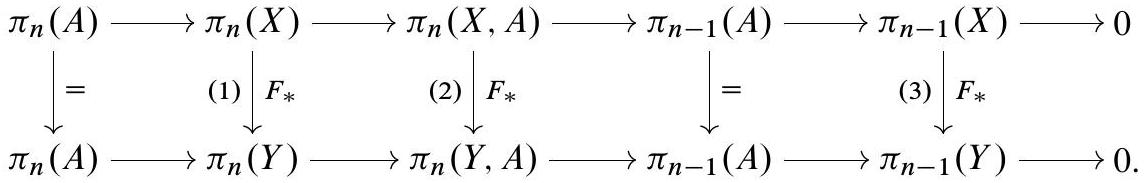
\includegraphics[scale=0.3,center]{2025_08_12_ad5732f7678306ae2ee7g-225}

The sequences end with 0 , since $\pi_{n-1}(X, A)=0$ and $\pi_{n-1}(A) \rightarrow \pi_{n-1}(Y)$ is surjective by assumption. (2) is surjective. The Five Lemma shows us that (1) is surjective and (3) injective. By induction hypothesis, (3) is already surjective. Hence $F$ is $n$-connected.

In order to obtain $A$ as a subcomplex of $X$, one works with cellular attaching maps.\\
(8.6.2) Theorem. Let $Y$ be a $C W$-complex such that $\pi_{i}(Y)=0$ for $0 \leq i \leq k$. Then $Y$ is homotopy equivalent to a $C W$-complex $X$ with $X^{k}=\{*\}$.

Proof. Start with the $k$-connected map $f: A=\{*\} \rightarrow Y$ and extend it to a weak equivalence $F: X \rightarrow Y$ by attaching cells of dimension greater than $k$.\\
(8.6.3) Proposition. Let $A$ and $B$ be pointed $C W$-complexes. Assume that $A$ is ( $m-1$ )-connected and $B$ is $(n-1)$-connected. Then $A \wedge_{k} B$ is $(m+n-1)$ connected.

Proof. We can assume that $A$ has no cells in dimensions less than $m$ and $n$ no cells in dimensions less than $n$ (except the base point). Then $A \wedge_{k} B$ has no cells in dimensions less than $m+n$.\\
(8.6.4) Theorem. Let ( $X_{j} \mid j \in J$ ) be afamily of ( $n-1$ )-connected $C W$-complexes. Let $\iota_{k}: X_{k} \rightarrow \bigvee_{j \in J} X_{j}$ be the inclusion of the $k$-th summand. Then

$$
\alpha_{J}=\left\langle\iota_{j *}:\right\rangle \bigoplus_{j \in J} \pi_{n}\left(X_{j}\right) \rightarrow \pi_{n}\left(\bigvee_{j \in J} X_{j}\right)
$$

is an isomorphism ( $n \geq 2$ ).\\
Proof. Let $J$ be finite. Up to h-equivalence we can assume that $X_{j}$ has no cells in dimensions less than $n$, except the base point. Then $\prod_{j} X_{j}$ is obtained from $\bigvee_{j} X_{j}$ by attaching cells of dimension $\geq 2 n$. Hence $\pi_{m}\left(\bigvee X_{j}\right) \rightarrow \pi_{m}\left(\prod X_{j}\right)$ is an isomorphism for $m \leq 2 n-2$. From the diagram\\
\includegraphics[scale=0.3,center]{2025_08_12_ad5732f7678306ae2ee7g-226}\\
we conclude that $\alpha_{J}$ is an isomorphism.\\
Let now $J$ be arbitrary. For each $x \in \pi_{n}\left(\bigvee_{j \in J} X_{j}\right)$ there exists a finite $E \subset J$ such that $x$ is contained in the image of $\pi_{n}\left(\bigvee_{E} X_{j}\right) \rightarrow \pi_{n}\left(\bigvee_{J} X_{j}\right)$, since a compact subset is contained in a finite wedge. The result for $E$ now shows that $\alpha_{J}$ is surjective. If $x_{1}$ and $x_{2}$ have the same image under $\alpha_{J}$, then these elements are contained in some finite sum $\bigoplus_{E}$ and, again by a compactness argument, they have the same image under some $\alpha_{E}$, if $E$ is chosen large enough. This shows the injectivity of $\alpha_{J}$.\\
(8.6.5) Proposition. Suppose $\pi_{j}(Y)=0$ for $j>n$. Let $X$ be obtained from $A$ by attaching cells of dimension $\geq n+2$. Then $A \subset X$ induces a bijection $[X, Y] \rightarrow[A, Y]$.

Proof. Surjective. Let $f: A \rightarrow Y$ be given. Attach $(n+2)$-cells via maps $\varphi: S^{n+1} \rightarrow A$. Since $f \varphi: S^{n+1} \rightarrow Y$ is null homotopic, we can extend $f$ over the ( $n+2$ )-cells. Continue in this manner.

Injective. Use the same argument for ( $X \times I, X \times \partial I \cup A \times I$ ). The cells of this relative complex have a dimension $>n+2$.\\
(8.6.6) Theorem. Let $A$ be an arbitrary space and $k \in \mathbb{N}_{0}$. There exists a relative $C W$-complex $(X, A)$ with cells only in dimensions $j \geq k+2$, such that $\pi_{n}(X, x)=0$ for $n>k$ and $x \in X$, and the induced map $\pi_{n}(A, a) \rightarrow \pi_{n}(X, a)$ is an isomorphism for $n \leq k$ and $a \in A$.

Proof. We construct inductively for $t \geq 2$ a sequence $A=X^{k+1} \subset X^{k+2} \subset$ $\cdots \subset X^{k+t}$ such that $\pi_{n}(A, a) \cong \pi_{n}\left(X^{k+t}, a\right)$ for $n \leq k, \pi_{n}\left(X^{k+t}, a\right)=0$ for $k<n \leq k+t-1$, and $X^{m+1}$ is obtained from $X^{m}$ by attaching ( $m+1$ )-cells.

The induction step: If we attach ( $m+1$ )-cells to $X^{m}$ by the attaching maps $\varphi_{j}:\left(S_{j}^{m}, e_{0}\right) \rightarrow\left(X^{m}, a\right)$ to obtain $X^{m+1}$, then $\pi_{n}\left(X^{m}, a\right) \cong \pi_{n}\left(X^{m+1}, a\right)$ for $n \leq m-1$. The exact sequence

$$
\pi_{m+1}\left(X^{m+1}, X^{m}, a\right) \xrightarrow{\partial} \pi_{m}\left(X^{m}, a\right) \rightarrow \pi_{m}\left(X^{m+1}, a\right) \rightarrow 0
$$

shows that the $\left[\varphi_{j}\right]$ are in the image of $\partial$. Thus, if the $\left[\varphi_{j}\right]$ generate $\pi_{m}\left(X^{m}, a\right)$, then $\pi_{m}\left(X^{m+1}, a\right)=0$.\\
(8.6.7) Example. We can attach cells of dimension $\geq n+2$ to $S^{n}$ to obtain a space $K(\mathbb{Z}, n)$ which has a single non-trivial homotopy group $\pi_{n}(K(\mathbb{Z}, n)) \cong \mathbb{Z}$. See the section on Eilenberg-Mac Lane spaces for a generalization.

Let $i_{n}^{X}: X \rightarrow X[n]$ be an inclusion of the type constructed in (8.6.6), namely $X[n]$ is obtained by attaching cells of dimension greater than $n+1$ such that $\pi_{k}(X[n])=0$ for $k>n$ and $i_{n}^{X}$ induces an isomorphism $\pi_{k}\left(i_{n}^{X}\right)$ for $k \leq n$. Given a map $f: X \rightarrow Y$ and $i_{m}^{Y}: Y \rightarrow Y[m]$ for $m \leq n$, there exists a unique homotopy class $f_{n, m}: X[n] \rightarrow Y[m]$ such that $i_{m}^{Y} \circ f=f_{n, m} \circ i_{n}^{X}$; this is a consequence of (8.6.5). We let $j_{n}^{X}: X\langle n\rangle \rightarrow X$ be the homotopy fibre of $i_{n}^{X}$. We call $j_{n}^{X}$ the $\boldsymbol{n}$-connective covering of $X$. The induced map $\pi_{i}\left(j_{n}^{X}\right): \pi_{i}(X\langle n\rangle) \rightarrow \pi_{i}(X)$ is an isomorphism for $i>n$ and $\pi_{i}(X\langle n\rangle)=0$ for $i \leq n$. The universal covering has such properties in the case that $n=1$. So we have a generalization, in the realm of fibrations. Objects of this type occur in the theory of Postnikov decompositions of a space, see e.g., [192].

As a consequence of (8.6.1) for $A=\emptyset$ we see that for each space $Y$ there exists a $C W$-complex $X$ and a weak equivalence $f: X \rightarrow Y$. We call such a weak\\
equivalence a CW-approximation of $Y$. Note that a weak equivalence between CWcomplexes is a homotopy equivalence (8.4.3). We show that CW-approximations are unique up to homotopy and functorial in the homotopy category.\\
(8.6.8) Theorem. Let $f: Y_{1} \rightarrow Y_{2}$ be a continuous map and let $\alpha_{j}: X_{j} \rightarrow Y_{j}$ be $C W$-approximations. Then there exists a map $\varphi: X_{1} \rightarrow X_{2}$ such that $f \alpha_{1} \simeq \alpha_{2} \varphi$, and the homotopy class of $\varphi$ is uniquely determined by this property.

Proof. Since $\alpha_{2}$ is a weak equivalence, $\alpha_{2}:\left[X_{1}, X_{2}\right] \rightarrow\left[X_{1}, Y_{2}\right]$ is bijective. Hence there exists a unique homotopy class $\varphi$ such that $f \alpha_{1} \simeq \alpha_{2} \varphi$.

A domination of $X$ by $K$ consists of maps $i: X \rightarrow K, p: K \rightarrow X$ and a homotopy pi $\simeq \operatorname{id}(X)$.\\
(8.6.9) Proposition. Suppose $M$ is dominated by a $C W$-complex $X$. Then $M$ has the homotopy type of a CW-complex.

Proof. Suppose $i: M \rightarrow X$ and $r: X \rightarrow M$ are given such that $r i$ is homotopic to the identity. There exists a CW-complex $\iota: X \subset Y$ and an extension $R: Y \rightarrow M$ of $r$ such that $R$ induces an isomorphism of homotopy groups. Let $j=i i: M \rightarrow$ $X \rightarrow Y$. Since $R j=r i \simeq \mathrm{id}$, the composition $R j$ induces isomorphisms of homotopy groups, hence so does $j$. From $j R j \simeq j$ we conclude that $j R$ induces the identity on homotopy groups and is therefore a homotopy equivalence. Let $k$ be h-inverse to $j R$, then $j(R k) \simeq \mathrm{id}$. Hence $j$ has the left inverse $R$ and the right inverse $R k$ and is therefore a homotopy equivalence.

A (half-exact) homotopy functor on the category $C^{0}$ of pointed connected CWspaces is a contravariant functor $h: C^{0} \rightarrow \mathrm{SET}^{0}$ into the category of pointed sets with the properties:\\
(1) (Homotopy invariance) Pointed homotopic maps induce the same morphism.\\
(2) (Mayer-Vietoris property) Suppose $X$ is the union of subcomplexes $A$ and $B$. If $a \in h(A)$ and $b \in h(B)$ are elements with the same restriction in $h(A \cap B)$, then there exists an element $x \in h(X)$ with restrictions $a$ and $b$.\\
(3) (Additivity) Let $X=\bigvee_{j} X_{j}$ with inclusions $i_{j}: X_{j} \rightarrow X$. Then

$$
h(X) \rightarrow \prod_{j} h\left(X_{j}\right), \quad x \mapsto\left(h\left(i_{j}\right) x\right)
$$

is bijective.\\
(8.6.10) Theorem (E. H. Brown). For each homotopy functor $h: C^{0} \rightarrow \mathrm{SET}^{0}$ there exist $K \in C^{0}$ and $u \in h(K)$ such that

$$
[X, K]^{0} \rightarrow h(X), \quad[f] \mapsto f^{*}(u)
$$

is bijective for each $X \in C^{0}$.

In category theory one says that $K$ is a representing object for the functor $h$. The theorem is called the representability theorem of E. H. Brown. For a proof see [31], [4].\\
(8.6.11) Example. Let $h(X)=[X, Z]^{0}$ for a connected pointed space $Z$. Then $h$ is a homotopy functor. From (8.6.10) we obtain $K \in C^{0}$ and $f: K \rightarrow Z$ such that $f_{*}:[X, K]^{0} \rightarrow[X, Z]^{0}$ is always bijective, i.e., $f$ is a weak h-equivalence. Thus we have obtained a CW-approximation $X$ of $Z$.

\section*{Problems}
\begin{enumerate}
  \item As a consequence of (8.6.8) one can extend homotopy functors from CW-complexes to arbitrary spaces. Let $F$ be a functor from the category of CW-complexes such that homotopic maps $f \simeq g$ induce the same morphism $F(f)=F(g)$. Then there is, up to natural isomorphism, a unique extension of $F$ to a homotopy invariant functor on TOP which maps weak equivalences to isomorphisms.
  \item A point is a $C W$-approximation of the pseudo-circle.
  \item Determine the $C W$-approximation of $\{0\} \cup\left\{n^{-1} \mid n \in \mathbb{N}\right\}$.
  \item Let $X$ and $Y$ be CW-complexes. Show that the identity $X \times_{k} Y \rightarrow X \times Y$ is a CWapproximation.
  \item Let ( $Y_{j} \mid j \in J$ ) be a family of well-pointed spaces and $\alpha_{j}: X_{j} \rightarrow Y_{j}$ a family of pointed CW-approximations. Then $\bigvee_{j} \alpha_{j}$ is a CW-approximation. Give a counterexample (with two spaces) in the case that the spaces are not well-pointed.
  \item Let $f: A \rightarrow B$ and $g: C \rightarrow D$ be pointed weak homotopy equivalences between wellpointed spaces. Then $f \wedge g$ is a weak homotopy equivalence.
  \item Verify from the axioms of a homotopy functor that $h(P)$ for a point $P$ contains a single element.
  \item Verify from the axioms of a homotopy functor that for each inclusion $A \subset X$ in $C^{0}$ the canonical sequence $h(X / A) \rightarrow h(X) \rightarrow h(A)$ is an exact sequence of pointed sets.
\end{enumerate}

\subsection*{Homotopy Classification}
In favorable cases the homotopy class of a map is determined by its effect on homotopy groups.\\
(8.7.1) Theorem. Let $X$ be an ( $n-1$ )-connected pointed $C W$-complex. Let $Y$ be a pointed space such that $\pi_{i}(Y)=0$ for $i>n \geq 2$. Then

$$
h_{X}:[X, Y]^{0} \rightarrow \operatorname{Hom}\left(\pi_{n}(X), \pi_{n}(Y)\right), \quad[f] \mapsto f_{*}
$$

is bijective.\\
Proof. The assertion only depends on the pointed homotopy type of $X$. We use (8.6.2) and assume $X^{n-1}=\{*\}$. The $h_{X}$ constitute a natural transformation in the variable $X$. Since ( $X, X^{n+1}$ ) is ( $n+1$ )-connected, the inclusion $X^{n+1} \subset X$ induces\\
an isomorphism on $\pi_{n}$. By (8.6.5), the restriction $r:[X, Y]^{0} \rightarrow\left[X^{n+1}, Y\right]^{0}$ is a bijection. Therefore it suffices to consider the case, that $X$ has, apart from the base point, only cells of dimension $n$ and $n+1$. Moreover, by the homotopy theorem for cofibrations, we can assume that the attaching maps for the $(n+1)$-cells are pointed. In this case $X$ is the mapping cone of a pointed map $f: A=\bigvee S_{k}^{n} \rightarrow \bigvee S_{j}^{n}=B$. We therefore have the exact cofibre sequence

$$
[A, Y]^{0} \stackrel{f^{*}}{\longleftarrow}[B, Y]^{0} \leftarrow[X, Y]^{0} \leftarrow[\Sigma A, Y]^{0} .
$$

Our assumption about $Y$ yields $[\Sigma A, Y]^{0}=\left[\bigvee \Sigma S_{k}^{n}, Y\right]^{0} \cong \prod_{k} \pi_{n+1}(Y)=0$. We apply the natural transformation $h$ and obtain a commutative diagram\\
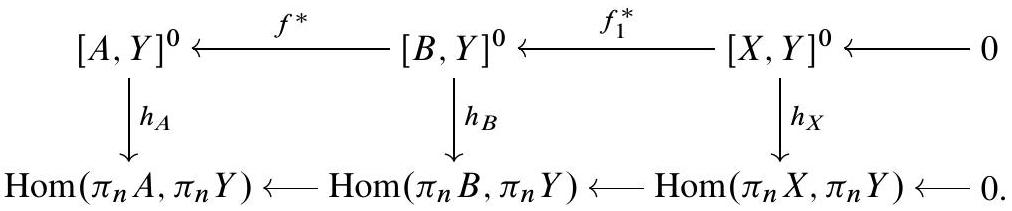
\includegraphics[scale=0.3,center]{2025_08_12_ad5732f7678306ae2ee7g-230(1)}

As one of the consequences of the excision theorem we showed that the sequence $\pi_{n}(A) \rightarrow \pi_{n}(B) \rightarrow \pi_{n}(X) \rightarrow 0$ is exact, and therefore the bottom sequence of the diagram is exact. We show that $h_{A}$ and $h_{B}$ are isomorphisms. If $A=S^{n}$, then

$$
h_{A}: \pi_{n}(Y)=\left[S^{n}, Y\right]^{0} \rightarrow \operatorname{Hom}\left(\pi_{n}\left(S^{n}\right), \pi_{n}(Y)\right)
$$

is an isomorphism, since $\pi_{n}\left(S^{n}\right)$ is generated by the identity. In the case that $A=\bigvee S_{k}^{n}$, we have a commutative diagram\\
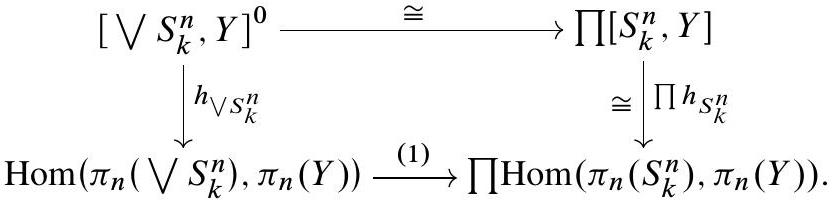
\includegraphics[scale=0.3,center]{2025_08_12_ad5732f7678306ae2ee7g-230}

The map (1) is induced by the isomorphism $\bigoplus \pi_{n}\left(S_{k}^{n}\right) \cong \pi_{n}\left(\bigvee S_{k}^{n}\right)$ and therefore an isomorphism. We now want to conclude from the diagram by a Five Lemma type argument that $h_{X}$ is bijective. The proof of surjectivity does not use the group structure. Injectivity follows, if $f_{1}^{*}$ is injective. In order to see this, one can use the general fact that $[\Sigma A, Y]^{0}$ acts on $[X, Y]^{0}$ and the orbits are mapped injectively, or one uses that $f$ is, up to homotopy, a suspension, because $\Sigma_{*}:\left[\bigvee S_{k}^{n-1}, \bigvee S_{j}^{n-1}\right]^{0} \rightarrow\left[\bigvee S_{k}^{n}, \bigvee S_{j}^{n}\right]^{0}$ is surjective.

\subsection*{Eilenberg-Mac Lane Spaces}
Let $\pi$ be an abelian group. An Eilenberg-Mac Lane space of type $\boldsymbol{K}(\boldsymbol{\pi}, \boldsymbol{n})$ is a CW-complex $K(\pi, n)$ such that $\pi_{n}(K(\pi, n)) \cong \pi$ and $\pi_{j}(K(\pi, n)) \cong 0$ for $j \neq n$.

In the cases $n=0,1$, the group $\pi$ can be non-abelian. In the case $n=0$, we think of $K(\pi, 0)=\pi$ with the discrete topology.\\
(8.8.1) Theorem. Eilenberg-Mac Lane spaces $K(\pi, n)$ exist.

Proof. Let $n \geq 2$. There exists an exact sequence

$$
0 \longrightarrow F_{1} \xrightarrow{\alpha} F_{0} \xrightarrow{\beta} \pi \longrightarrow 0
$$

with free abelian groups $F_{0}$ and $F_{1}$. We fix a basis ( $a_{k} \mid k \in K$ ) of $F_{1}$ and $\left(b_{j} \mid j \in J\right)$ of $F_{0}$. Then $\alpha$ is determined by the matrix $\alpha\left(a_{k}\right)=\sum_{j} n(j, k) b_{j}$. We now construct a geometric realization of this algebraic situation. The group $\pi_{n}\left(\bigvee_{k} S_{k}^{n}\right) \cong \bigoplus_{k} \pi_{n}\left(S_{k}^{n}\right)$ is free abelian (8.6.4). A basis is given by the canonical inclusions $S_{l}^{n} \rightarrow \bigvee S_{k}^{n}$. There exists a unique homotopy class $f: A=\bigvee_{k} S_{k}^{n} \rightarrow$ $\bigvee S_{j}^{n}=B$ which realizes the matrix ( $n(j, k)$ ) with respect to these bases. Let $X=C(f)$ be the mapping cone of $f$. Then the sequence

$$
\pi_{n}(A) \xrightarrow{f_{*}} \pi_{n}(B) \xrightarrow{f_{1 *}} \pi_{n}(X) \longrightarrow 0
$$

is exact. Hence $\pi_{n}(X) \cong \pi$. Also $\pi_{i}(X)=0$ for $i<n$. We can now attach cells of dimensions $\geq n+2$ to $X$ in order to obtain a $K(\pi, n)$, see (8.6.6).\\
(8.8.2) Examples. The space $S^{1}$ is a $K(\mathbb{Z}, 1)$. We know $\pi_{1}\left(S^{1}\right) \cong \mathbb{Z}$, and from the exact sequence of the universal covering $\mathbb{R} \rightarrow S^{1}$ we know that $\pi_{n}\left(S^{1}\right)=0$ for $n \geq 2$. The space $\mathbb{C} P^{\infty}$ is a model for $K(\mathbb{Z}, 2)$. The space $\mathbb{R} P^{\infty}$ is a $K(\mathbb{Z} / 2,1)$.

The adjunction $[\Sigma X, Y]^{0} \cong[X, \Omega Y]^{0}$ shows that $\Omega K(\pi, n+1)$ has the homotopy groups of a $K(\pi, n)$. By a theorem of Milnor [132], [67], $\Omega Y$ has the homotopy type of a CW-complex if $Y$ is a CW-complex. If one does not want to use this result one has the weaker result that there exists a weak homotopy equivalence $K(\pi, n) \rightarrow \Omega K(\pi, n+1)$.

We now establish further properties of Eilenberg-Mac Lane spaces. We begin by showing that Eilenberg-Mac Lane spaces are $H$-spaces. Then we construct product pairings $K(\pi, m) \wedge K(\rho, n) \rightarrow K(\pi \otimes \rho, m+n)$. In this context $\pi \otimes \rho$ denotes the tensor product of the abelian groups $\pi$ and $\rho$ (alias $\mathbb{Z}$-modules) over $\mathbb{Z}$.

We call the space $K(\pi, n)$ polarized, if we have chosen a fixed isomorphism $\alpha: \pi_{n}(K(\pi, n)) \rightarrow \pi$. If ( $K(\pi, n), \alpha$ ) and ( $K(\rho, n), \beta$ ) are polarized complexes, the product $K(\pi, n) \times K(\rho, n)$ will be polarized by

$$
\pi_{n}(K(\pi, n) \times K(\rho, n)) \cong \pi_{n}(K(\pi, n)) \times \pi_{n}(K(\rho, n)) \xrightarrow{\alpha \times \beta} \pi_{1} \times \pi_{2} .
$$

(8.8.3) Proposition. Having chosen polarizations, we obtain from (8.7.1) an isomorphism $[K(\pi, n), K(\rho, n)]^{0} \cong \operatorname{Hom}(\pi, \rho)$.\\
(8.8.4) Theorem. Let $\pi$ be an abelian group. Then an Eilenberg-Mac Lane complex $K(\pi, n)$ is a commutative group object in h -TOP.

Proof. Let $K=(K(\pi, n), \alpha)$ be a polarized complex with base point a 0 -cell $e$. For an abelian group $\pi$, the multiplication $\mu: \pi \times \pi \rightarrow \pi,(g, h) \mapsto g h$ is a homomorphism. Therefore there exists a map $m: K \times K \rightarrow K$, unique up to homotopy, which corresponds under (8.8.3) to $\mu$. Similarly, $l: \pi \rightarrow \pi, g \mapsto g^{-1}$ is a homomorphism and yields a map $i: K \rightarrow K$. Claim: $(K, m, i)$ is an associative and commutative $H$-space. The maps $m \circ(m \times \mathrm{id})$ and $m \circ(\mathrm{id} \times m)$ induce the same homomorphism when $\pi_{n}$ is applied; hence these maps are homotopic. In a similar manner one shows that $x \mapsto m(x, e)$ is homotopic to the identity. Since $K \vee K \subset K \times K$ is a cofibration, we can change $m$ by a homotopy such that $m(x, e)=m(e, x)=x$. We write $x \mapsto m(x, i(x))$ as composition

$$
K \xrightarrow{d} K \times K \xrightarrow{\text { id } \times i} K \times K \xrightarrow{m} K
$$

and apply $\pi_{n}$; the result is the constant homomorphism. Hence this map is null homotopic. Commutativity is verified in a similar manner by applying $\pi_{n}$. See also Problem 1.

For the construction of the product pairing we need a general result about products for homotopy groups. We take the smash product of representatives $f: I^{m} / \partial I^{m} \rightarrow X, g: I^{n} / \partial I^{n} \rightarrow Y$ and obtain a well-defined map

$$
\pi_{m}(X) \times \pi_{n}(Y) \rightarrow \pi_{m+n}\left(X \wedge_{k} Y\right), \quad([f],[g]) \mapsto[f \wedge g]=[f] \wedge[g] .
$$

We call this map the $\wedge$-product for homotopy groups. It is natural in the variables $X$ and $Y$.\\
(8.8.5) Proposition. The $\wedge$-product is bi-additive.

Proof. The additivity in the first variable follows directly from the definition of the addition, if we use $+_{1}$. We see the additivity in the second variable, if we use the composition laws $+_{1}$ and $+_{m+1}$ in the homotopy groups.\\
(8.8.6) Proposition. Let $A$ be an ( $m-1$ )-connected and $B$ an ( $n-1$ )-connected $C W$-complex. Then $A \wedge B$ is ( $m+n-1$ )-connected and the $\wedge$-product

$$
\pi_{m}(A) \otimes \pi_{n}(B) \rightarrow \pi_{m+n}\left(A \wedge_{k} B\right)
$$

is an isomorphism ( $m, n \geq 2$ ). If $m$ or $n$ equals 1 , then one has to use the abelianized groups.

Proof. The assertion about the connectivity was shown in (8.6.3). For $A=S^{m}$ the assertion holds by the suspension theorem. For $A=\bigvee_{j} S_{j}^{m}$ we use the commutative diagram\\
\includegraphics[scale=0.3,center]{2025_08_12_ad5732f7678306ae2ee7g-233(1)}\\
(1) is an isomorphism by (8.6.4). (2) is induced by a homeomorphism. (3) is an isomorphism by algebra. (4) is an isomorphism by (8.6.4). (5) is an isomorphism by the suspension theorem. This settles the case of a wedge of $m$-spheres. Next we let $A$ be the mapping cone of a map $f: C \rightarrow D$ where $C$ and $D$ are wedges of $m$-spheres. Then we have a commutative diagram with exact rows:\\
\includegraphics[scale=0.3,center]{2025_08_12_ad5732f7678306ae2ee7g-233(2)}

The general case now follows from the observation that the inclusion $A^{m+1} \rightarrow A$ induces an isomorphism on $\pi_{m}$ and $A^{m+1} \wedge_{k} B \rightarrow A \wedge_{k} B$ induces an isomorphism on $\pi_{m+n}$.

Let $(K(G, m), \alpha),(K(H, n), \beta)$ and $(K(G \otimes H, m+n), \gamma)$ be polarized Eilen-berg-Mac Lane complexes for abelian groups $G$ and $H$. A product is a map

$$
\gamma_{m, n}: K(G, m) \wedge_{k} K(H, n) \rightarrow K(G \otimes H, m+n)
$$

such that the diagram\\
\includegraphics[scale=0.3,center]{2025_08_12_ad5732f7678306ae2ee7g-233}\\
is commutative. Here we have use the $\wedge$-product (8.8.5).\\
(8.8.7) Theorem. There exists a product. It is unique up to homotopy.

Proof. Let $G$ and $H$ be abelian groups. The first non-trivial homotopy group of $K(G, m) \wedge_{k} K(H, n)$ is $\pi_{m+n}$ and it is isomorphic to $G \otimes H$, see (8.8.6). By (8.6.6) there exists an inclusion

$$
\gamma_{m, n}: K(G, m) \wedge_{k} K(H, n) \rightarrow K(G \otimes H, m+n) .
$$

We can choose the polarization $\gamma$ so that the diagram above becomes commutative. Uniqueness follows from (8.7.1).

The products (8.8.7) are associative, i.e.,

$$
\gamma_{m+n, p} \circ\left(\gamma_{m, n} \times \mathrm{id}\right) \simeq \gamma_{m, n+p} \circ\left(\mathrm{id} \times \gamma_{n, p}\right) .
$$

The products are graded commutative in the following sense:

$$
K(\tau, m+n) \circ \gamma_{m, n} \simeq(-1)^{m n} \tau^{\prime} \circ \gamma_{n, m}
$$

with the interchange maps $\tau^{\prime}: K(m, G) \wedge K(n, H) \rightarrow K(n, H) \wedge K(m, G)$ and $\tau: G \otimes H \rightarrow H \otimes G$.

Let $R$ be a commutative ring with 1 . We think of the multiplication as being a homomorphism $\mu: R \otimes R \rightarrow R$ between abelian groups. From this homomorphism we obtain a unique homotopy class $K(\mu): K(R \otimes R, m) \rightarrow K(R, m)$.

We compose $K(\mu)$ with $\gamma_{k, l}$ and obtain a product map

$$
m_{k, l}: K(R, k) \wedge_{k} K(R, l) \rightarrow K(R, k+l) .
$$

Also these products are associative and graded commutative.\\
In the associated homotopy groups $H^{k}(X ; R)=\left[X^{+}, K(R, k)\right]^{0}$ we obtain via $(f, g) \mapsto m_{k, l}(f \wedge g)$ products

$$
H^{k}(X ; R) \otimes H^{l}(Y ; R) \rightarrow H^{k+l}(X \times Y ; R),
$$

which are also associative and graded commutative. (See also Problem 3.) In a similar manner we can start from an $R$-module structure $R \otimes M \rightarrow M$ on $M$. Later, when we study singular cohomology, we show that for a CW-complex $X$ the group $\left[X^{+}, K(R, k)\right]^{0}$ is naturally isomorphic to the singular cohomology group $H^{k}(X ; R)$ with coefficients in the ring $R$. This opens the way to a homotopical study of cohomology. The product (8.8.7) can then be used to construct the so-called cup product in cohomology.

Once singular cohomology theory is constructed one obtains from the representability theorem of Brown Eilenberg-Mac Lane spaces as representing objects.\\
8.8.8 Eilenberg-Mac Lane spectra. Let $A$ be an abelian group. The EilenbergMac Lane spectrum $H A$ consists of the family $\left(K(A, n) \mid n \in \mathbb{N}_{0}\right)$ of EilenbergMac Lane CW-spaces and maps $e_{n}: \Sigma K(A, n) \rightarrow K(A, n+1)$ (an inclusion of\\
subcomplexes; attach cells to $\Sigma K(A, n)$ to obtain a $K(A, n+1))$. This spectrum is an $\Omega$-spectrum. We have proved in any case that $\varepsilon_{n}: K(A, n) \rightarrow \Omega K(A, n+1)$ is a weak homotopy equivalence. This suffices if one wants to define the cohomology theory only for pointed CW-spaces.

\section*{Problems}
\begin{enumerate}
  \item From the natural isomorphism $[X, K(\pi, n)]^{0} \cong\left[X, \Omega^{2} K(\pi, n+2)\right]^{0}$ we see that $X \mapsto$ $[X, K(\pi, n)]^{0}$ is a contravariant functor into the category of abelian groups. Therefore, by category theory, there exists a unique (up to homotopy) structure of a commutative h-group on $K(\pi, n)$ inducing the group structures of this functor.
  \item Let $\alpha \in \pi_{m}(X), \beta \in \pi_{n}(Y)$, and $\tau: X \wedge_{k} Y \rightarrow Y \wedge_{k} X$ the interchange map. Then $\alpha \wedge \beta=(-1)^{m n} \beta \wedge \alpha$.
  \item Let $M$ be an $R$-module. A left translation $l_{r}: M \rightarrow M, x \mapsto r x$ is a homomorphism of the abelian group $M$ and induces therefore a map $L_{r}: K(M, k) \rightarrow K(M, k)$. Use these maps to define a natural structure of an $R$-module on $[X, K(M, k)]^{0}$.
  \item The simply connected surfaces are $S^{2}$ and $\mathbb{R}^{2}$ [44, p. 87]. If a surface is different from $S^{2}$ and $\mathbb{R} P^{2}$, then it is a $K(\pi, 1)$.
  \item Let $E(\pi) \rightarrow B(\pi)$ be a $\pi$-principal covering with contractible $E(\pi)$. Then $B(\pi)$ is a $K(\pi, 1)$. Spaces of the type $B(\pi)$ will occur later as classifying spaces. There is a bijection $[K(\pi, 1), K(\rho, 1)] \cong \operatorname{Hom}(\pi, \rho) / \sim$ between homotopy classes and group homomorphisms up to inner automorphisms.
  \item Let $S^{\infty}$ be the colimit of the unit spheres $S\left(\mathbb{C}^{n}\right) \subset S\left(\mathbb{C}^{n+1}\right) \subset \cdots$. This space carries a free action of the cyclic group $\mathbb{Z} / m \subset S^{1}$ by scalar multiplication. Show that $S^{\infty}$ with this action is a $\mathbb{Z} / m$-principal covering. The quotient space is a CW-space $B(\mathbb{Z} / m)$ and hence a $K(\mathbb{Z} / m, 1)$.
  \item A connected 1 -dimensional CW-complex $X$ is a $K(\pi, 1)$. Determine $\pi$ from the topology of $X$.
  \item A connected non-closed surface (with or without boundary) is a $K(\pi, 1)$.
\end{enumerate}





\pagebreak
\printbibliography
\end{document}